% Options for packages loaded elsewhere
\PassOptionsToPackage{unicode}{hyperref}
\PassOptionsToPackage{hyphens}{url}
%
\documentclass[
  11pt,
]{article}
\usepackage{amsmath,amssymb}
\usepackage{lmodern}
\usepackage{iftex}
\ifPDFTeX
  \usepackage[T1]{fontenc}
  \usepackage[utf8]{inputenc}
  \usepackage{textcomp} % provide euro and other symbols
\else % if luatex or xetex
  \usepackage{unicode-math}
  \defaultfontfeatures{Scale=MatchLowercase}
  \defaultfontfeatures[\rmfamily]{Ligatures=TeX,Scale=1}
\fi
% Use upquote if available, for straight quotes in verbatim environments
\IfFileExists{upquote.sty}{\usepackage{upquote}}{}
\IfFileExists{microtype.sty}{% use microtype if available
  \usepackage[]{microtype}
  \UseMicrotypeSet[protrusion]{basicmath} % disable protrusion for tt fonts
}{}
\makeatletter
\@ifundefined{KOMAClassName}{% if non-KOMA class
  \IfFileExists{parskip.sty}{%
    \usepackage{parskip}
  }{% else
    \setlength{\parindent}{0pt}
    \setlength{\parskip}{6pt plus 2pt minus 1pt}}
}{% if KOMA class
  \KOMAoptions{parskip=half}}
\makeatother
\usepackage{xcolor}
\usepackage[margin=1in]{geometry}
\usepackage{color}
\usepackage{fancyvrb}
\newcommand{\VerbBar}{|}
\newcommand{\VERB}{\Verb[commandchars=\\\{\}]}
\DefineVerbatimEnvironment{Highlighting}{Verbatim}{commandchars=\\\{\}}
% Add ',fontsize=\small' for more characters per line
\newenvironment{Shaded}{}{}
\newcommand{\AlertTok}[1]{\textcolor[rgb]{1.00,0.00,0.00}{#1}}
\newcommand{\AnnotationTok}[1]{\textcolor[rgb]{0.00,0.50,0.00}{#1}}
\newcommand{\AttributeTok}[1]{#1}
\newcommand{\BaseNTok}[1]{#1}
\newcommand{\BuiltInTok}[1]{#1}
\newcommand{\CharTok}[1]{\textcolor[rgb]{0.00,0.50,0.50}{#1}}
\newcommand{\CommentTok}[1]{\textcolor[rgb]{0.00,0.50,0.00}{#1}}
\newcommand{\CommentVarTok}[1]{\textcolor[rgb]{0.00,0.50,0.00}{#1}}
\newcommand{\ConstantTok}[1]{#1}
\newcommand{\ControlFlowTok}[1]{\textcolor[rgb]{0.00,0.00,1.00}{#1}}
\newcommand{\DataTypeTok}[1]{#1}
\newcommand{\DecValTok}[1]{#1}
\newcommand{\DocumentationTok}[1]{\textcolor[rgb]{0.00,0.50,0.00}{#1}}
\newcommand{\ErrorTok}[1]{\textcolor[rgb]{1.00,0.00,0.00}{\textbf{#1}}}
\newcommand{\ExtensionTok}[1]{#1}
\newcommand{\FloatTok}[1]{#1}
\newcommand{\FunctionTok}[1]{#1}
\newcommand{\ImportTok}[1]{#1}
\newcommand{\InformationTok}[1]{\textcolor[rgb]{0.00,0.50,0.00}{#1}}
\newcommand{\KeywordTok}[1]{\textcolor[rgb]{0.00,0.00,1.00}{#1}}
\newcommand{\NormalTok}[1]{#1}
\newcommand{\OperatorTok}[1]{#1}
\newcommand{\OtherTok}[1]{\textcolor[rgb]{1.00,0.25,0.00}{#1}}
\newcommand{\PreprocessorTok}[1]{\textcolor[rgb]{1.00,0.25,0.00}{#1}}
\newcommand{\RegionMarkerTok}[1]{#1}
\newcommand{\SpecialCharTok}[1]{\textcolor[rgb]{0.00,0.50,0.50}{#1}}
\newcommand{\SpecialStringTok}[1]{\textcolor[rgb]{0.00,0.50,0.50}{#1}}
\newcommand{\StringTok}[1]{\textcolor[rgb]{0.00,0.50,0.50}{#1}}
\newcommand{\VariableTok}[1]{#1}
\newcommand{\VerbatimStringTok}[1]{\textcolor[rgb]{0.00,0.50,0.50}{#1}}
\newcommand{\WarningTok}[1]{\textcolor[rgb]{0.00,0.50,0.00}{\textbf{#1}}}
\usepackage{graphicx}
\makeatletter
\def\maxwidth{\ifdim\Gin@nat@width>\linewidth\linewidth\else\Gin@nat@width\fi}
\def\maxheight{\ifdim\Gin@nat@height>\textheight\textheight\else\Gin@nat@height\fi}
\makeatother
% Scale images if necessary, so that they will not overflow the page
% margins by default, and it is still possible to overwrite the defaults
% using explicit options in \includegraphics[width, height, ...]{}
\setkeys{Gin}{width=\maxwidth,height=\maxheight,keepaspectratio}
% Set default figure placement to htbp
\makeatletter
\def\fps@figure{htbp}
\makeatother
\setlength{\emergencystretch}{3em} % prevent overfull lines
\providecommand{\tightlist}{%
  \setlength{\itemsep}{0pt}\setlength{\parskip}{0pt}}
\setcounter{secnumdepth}{-\maxdimen} % remove section numbering
\ifLuaTeX
  \usepackage{selnolig}  % disable illegal ligatures
\fi
\IfFileExists{bookmark.sty}{\usepackage{bookmark}}{\usepackage{hyperref}}
\IfFileExists{xurl.sty}{\usepackage{xurl}}{} % add URL line breaks if available
\urlstyle{same} % disable monospaced font for URLs
\hypersetup{
  pdftitle={Appendix S3. Steps to recreate the manuscript figures.},
  hidelinks,
  pdfcreator={LaTeX via pandoc}}

\title{Appendix S3. Steps to recreate the manuscript figures.}
\author{}
\date{\vspace{-2.5em}}

\begin{document}
\maketitle

{
\setcounter{tocdepth}{3}
\tableofcontents
}
\vspace{0.2in}

This is version 0.23.02.17.

\newpage

\hypertarget{setup}{%
\section{Setup}\label{setup}}

This appendix shows how to recreate the figures in the main text based
on the results from the best of the fitted models. All analyses require
the \href{https://cran.r-project.org/}{R software} (v3.5 or later), as
well as a few packages that are not included with the base installation
of R.

\begin{Shaded}
\begin{Highlighting}[]
\FunctionTok{library}\NormalTok{(}\StringTok{"here"}\NormalTok{)}
\FunctionTok{library}\NormalTok{(}\StringTok{"readr"}\NormalTok{)}
\FunctionTok{library}\NormalTok{(}\StringTok{"captioner"}\NormalTok{)}
\FunctionTok{library}\NormalTok{(}\StringTok{"coda"}\NormalTok{)}
\FunctionTok{library}\NormalTok{(}\StringTok{"gsl"}\NormalTok{)}

\DocumentationTok{\#\# set default caption delimter}
\NormalTok{fig\_cap }\OtherTok{\textless{}{-}} \FunctionTok{captioner}\NormalTok{(}\AttributeTok{infix =} \StringTok{"."}\NormalTok{) }\CommentTok{\# I changed suffix to infix because it was producing an error}

\DocumentationTok{\#\# set directory locations}
\NormalTok{datadir }\OtherTok{\textless{}{-}} \FunctionTok{here}\NormalTok{(}\StringTok{"data"}\NormalTok{)}
\NormalTok{savedir }\OtherTok{\textless{}{-}} \FunctionTok{here}\NormalTok{(}\StringTok{"analysis/cache"}\NormalTok{)}

\DocumentationTok{\#\# round/floor/ceiling with varying precision}
\NormalTok{around }\OtherTok{\textless{}{-}} \ControlFlowTok{function}\NormalTok{(x, }\AttributeTok{func =} \StringTok{"round"}\NormalTok{, }\AttributeTok{prec =} \DecValTok{1}\NormalTok{) \{}
  \DocumentationTok{\#\# \textasciigrave{}x\textasciigrave{} must be a real number}
  \ControlFlowTok{if}\NormalTok{(}\SpecialCharTok{!}\FunctionTok{is.double}\NormalTok{(x)) \{}
    \FunctionTok{stop}\NormalTok{(}\StringTok{"\textasciigrave{}x\textasciigrave{} must be a real number"}\NormalTok{)}
\NormalTok{  \}}
  \DocumentationTok{\#\# \textasciigrave{}func\textasciigrave{} can be "round", "floor", or "ceiling"}
  \ControlFlowTok{if}\NormalTok{(}\SpecialCharTok{!}\NormalTok{(func }\SpecialCharTok{\%in\%} \FunctionTok{c}\NormalTok{(}\StringTok{"round"}\NormalTok{, }\StringTok{"floor"}\NormalTok{, }\StringTok{"ceiling"}\NormalTok{))) \{}
    \FunctionTok{stop}\NormalTok{(}\StringTok{"\textasciigrave{}func\textasciigrave{} must be one of }\SpecialCharTok{\textbackslash{}"}\StringTok{round}\SpecialCharTok{\textbackslash{}"}\StringTok{, }\SpecialCharTok{\textbackslash{}"}\StringTok{floor}\SpecialCharTok{\textbackslash{}"}\StringTok{, or }\SpecialCharTok{\textbackslash{}"}\StringTok{ceiling}\SpecialCharTok{\textbackslash{}"}\StringTok{"}\NormalTok{)}
\NormalTok{  \}}
  \DocumentationTok{\#\# \textasciigrave{}prec\textasciigrave{} is desired precision (eg, 0.1 is to nearest tenth)}
  \ControlFlowTok{if}\NormalTok{(prec }\SpecialCharTok{\textless{}=} \DecValTok{0}\NormalTok{) \{}
    \FunctionTok{stop}\NormalTok{(}\StringTok{"\textasciigrave{}prec\textasciigrave{} cannot be less than or equal to 0"}\NormalTok{)}
\NormalTok{  \}}
  \FunctionTok{do.call}\NormalTok{(func, }\FunctionTok{list}\NormalTok{(x }\SpecialCharTok{/}\NormalTok{ prec)) }\SpecialCharTok{*}\NormalTok{ prec}
\NormalTok{\}}
\end{Highlighting}
\end{Shaded}

\hypertarget{user-inputs}{%
\section{User inputs}\label{user-inputs}}

\begin{Shaded}
\begin{Highlighting}[]
\DocumentationTok{\#\# first \& last years of fish data}
\NormalTok{yr\_frst }\OtherTok{\textless{}{-}} \DecValTok{1978}
\NormalTok{yr\_last }\OtherTok{\textless{}{-}} \DecValTok{2018}
\DocumentationTok{\#\# years of data}
\NormalTok{dat\_yrs }\OtherTok{\textless{}{-}} \FunctionTok{seq}\NormalTok{(yr\_frst, yr\_last)}
\DocumentationTok{\#\# number of years of data}
\NormalTok{n\_yrs }\OtherTok{\textless{}{-}} \FunctionTok{length}\NormalTok{(dat\_yrs)}

\DocumentationTok{\#\# min \& max adult age classes}
\NormalTok{age\_min }\OtherTok{\textless{}{-}} \DecValTok{3}
\NormalTok{age\_max }\OtherTok{\textless{}{-}} \DecValTok{8}
\DocumentationTok{\#\# num of age classes}
\NormalTok{A }\OtherTok{\textless{}{-}}\NormalTok{ age\_max }\SpecialCharTok{{-}}\NormalTok{ age\_min }\SpecialCharTok{+} \DecValTok{1}

\DocumentationTok{\#\# posterior coverage interval}
\NormalTok{CI\_vec }\OtherTok{\textless{}{-}} \FunctionTok{c}\NormalTok{(}\FloatTok{0.025}\NormalTok{,}\FloatTok{0.5}\NormalTok{,}\FloatTok{0.975}\NormalTok{)}

\DocumentationTok{\#\# covariate names \& units for plotting}
\NormalTok{cov\_names }\OtherTok{\textless{}{-}} \FunctionTok{c}\NormalTok{(}\FunctionTok{expression}\NormalTok{(}\FunctionTok{paste}\NormalTok{(}\StringTok{"Max flow ("}\NormalTok{,m}\SpecialCharTok{\^{}}\DecValTok{3}\NormalTok{,}\StringTok{" "}\NormalTok{,s}\SpecialCharTok{\^{}}\NormalTok{\{}\SpecialCharTok{{-}}\DecValTok{1}\NormalTok{\},}\StringTok{")"}\NormalTok{)),}
               \FunctionTok{expression}\NormalTok{(}\FunctionTok{paste}\NormalTok{(}\StringTok{"Min flow ("}\NormalTok{,m}\SpecialCharTok{\^{}}\DecValTok{3}\NormalTok{,}\StringTok{" "}\NormalTok{,s}\SpecialCharTok{\^{}}\NormalTok{\{}\SpecialCharTok{{-}}\DecValTok{1}\NormalTok{\},}\StringTok{")"}\NormalTok{)),}
               \StringTok{"NPGO"}\NormalTok{,}
               \FunctionTok{expression}\NormalTok{(}\FunctionTok{paste}\NormalTok{(}\StringTok{"H releases ("}\NormalTok{,}\DecValTok{10}\SpecialCharTok{\^{}}\DecValTok{3}\NormalTok{,}\StringTok{")"}\NormalTok{)))}
\end{Highlighting}
\end{Shaded}

\hypertarget{load-the-information}{%
\section{Load the information}\label{load-the-information}}

Here we load in the estimated parameters and states from the selected
model, as well as the covariates and harvest data and escapement data.

\begin{Shaded}
\begin{Highlighting}[]
\DocumentationTok{\#\# best fitting model}
\NormalTok{best\_fit }\OtherTok{\textless{}{-}} \FunctionTok{readRDS}\NormalTok{(}\FunctionTok{file.path}\NormalTok{(savedir, }\StringTok{"fit\_bh\_cov.rds"}\NormalTok{))}

\DocumentationTok{\#\# covariate(s)}
\NormalTok{dat\_cvrs }\OtherTok{\textless{}{-}} \FunctionTok{read\_csv}\NormalTok{(}\FunctionTok{file.path}\NormalTok{(datadir, }\StringTok{"skagit\_sthd\_covars.csv"}\NormalTok{))}
\DocumentationTok{\#\# total number of covariates}
\NormalTok{n\_cov }\OtherTok{\textless{}{-}} \FunctionTok{dim}\NormalTok{(dat\_cvrs)[}\DecValTok{2}\NormalTok{] }\SpecialCharTok{{-}} \DecValTok{1}

\DocumentationTok{\#\# escapement}
\NormalTok{dat\_esc }\OtherTok{\textless{}{-}} \FunctionTok{read\_csv}\NormalTok{(}\FunctionTok{file.path}\NormalTok{(datadir, }\StringTok{"skagit\_sthd\_esc.csv"}\NormalTok{))}
\DocumentationTok{\#\# log of escapement}
\NormalTok{ln\_dat\_esc }\OtherTok{\textless{}{-}} \FunctionTok{log}\NormalTok{(dat\_esc}\SpecialCharTok{$}\NormalTok{escapement)}

\DocumentationTok{\#\# harvest}
\NormalTok{dat\_harv }\OtherTok{\textless{}{-}} \FunctionTok{read\_csv}\NormalTok{(}\FunctionTok{file.path}\NormalTok{(datadir, }\StringTok{"skagit\_sthd\_catch.csv"}\NormalTok{))}
\DocumentationTok{\#\# drop year col \& first age\_max rows}
\NormalTok{dat\_harv }\OtherTok{\textless{}{-}}\NormalTok{ dat\_harv}\SpecialCharTok{$}\NormalTok{catch}
\end{Highlighting}
\end{Shaded}

\hypertarget{main-results}{%
\section{Main results}\label{main-results}}

We need to convert the \texttt{mcmc.list} output into a more
user-friendly form for plotting, etc.

\begin{Shaded}
\begin{Highlighting}[]
\DocumentationTok{\#\# reformat model posteriors}
\NormalTok{mod\_res }\OtherTok{\textless{}{-}} \FunctionTok{do.call}\NormalTok{(}\StringTok{"rbind"}\NormalTok{, best\_fit)}
\end{Highlighting}
\end{Shaded}

\hypertarget{fig-1---model-forms}{%
\subsection{Fig 1 - Model forms}\label{fig-1---model-forms}}

Here are the model parameters we used for the schematics of the
deterministic forms for the Ricker and Beverton-Holt models.

\begin{Shaded}
\begin{Highlighting}[]
\DocumentationTok{\#\# params}
\DocumentationTok{\#\# Ricker}
\NormalTok{ra }\OtherTok{\textless{}{-}} \DecValTok{3}
\NormalTok{rb }\OtherTok{\textless{}{-}} \FloatTok{1.2e{-}4}
\DocumentationTok{\#\# B{-}H}
\NormalTok{ba }\OtherTok{\textless{}{-}} \DecValTok{3}
\NormalTok{bb }\OtherTok{\textless{}{-}} \DecValTok{3}\SpecialCharTok{/}\FloatTok{1.4e4}

\DocumentationTok{\#\# ref pts}
\DocumentationTok{\#\# Ricker}
\NormalTok{rmr }\OtherTok{\textless{}{-}}\NormalTok{ ra}\SpecialCharTok{/}\NormalTok{rb}\SpecialCharTok{*}\FunctionTok{exp}\NormalTok{(}\SpecialCharTok{{-}}\DecValTok{1}\NormalTok{)}
\NormalTok{rsy }\OtherTok{\textless{}{-}}\NormalTok{ (}\DecValTok{1} \SpecialCharTok{{-}} \FunctionTok{lambert\_W0}\NormalTok{(}\FunctionTok{exp}\NormalTok{(}\DecValTok{1}\NormalTok{)}\SpecialCharTok{/}\NormalTok{ra)) }\SpecialCharTok{/}\NormalTok{ rb}
\NormalTok{ruy }\OtherTok{\textless{}{-}} \DecValTok{1} \SpecialCharTok{{-}} \FunctionTok{lambert\_W0}\NormalTok{(}\FunctionTok{exp}\NormalTok{(}\DecValTok{1}\NormalTok{)}\SpecialCharTok{/}\NormalTok{ra)}
\DocumentationTok{\#\# B{-}H}
\NormalTok{bmr }\OtherTok{\textless{}{-}}\NormalTok{ ba}\SpecialCharTok{/}\NormalTok{bb}
\NormalTok{bsy }\OtherTok{\textless{}{-}}\NormalTok{ (ba}\SpecialCharTok{/}\NormalTok{bb)}\SpecialCharTok{*}\FunctionTok{sqrt}\NormalTok{(}\DecValTok{1}\SpecialCharTok{/}\NormalTok{ba)}\SpecialCharTok{{-}}\NormalTok{(}\DecValTok{1}\SpecialCharTok{/}\NormalTok{bb)}
\NormalTok{bsy }\OtherTok{\textless{}{-}}\NormalTok{ (}\FunctionTok{sqrt}\NormalTok{(ba)}\SpecialCharTok{{-}}\DecValTok{1}\NormalTok{)}\SpecialCharTok{/}\NormalTok{bb}
\NormalTok{buy }\OtherTok{\textless{}{-}} \DecValTok{1} \SpecialCharTok{{-}} \FunctionTok{sqrt}\NormalTok{(}\DecValTok{1}\SpecialCharTok{/}\NormalTok{ba)}

\DocumentationTok{\#\# S{-}R curves}
\DocumentationTok{\#\# spawners}
\NormalTok{ss }\OtherTok{\textless{}{-}} \FunctionTok{seq}\NormalTok{(}\DecValTok{0}\NormalTok{,}\FloatTok{1.2e4}\NormalTok{,}\DecValTok{10}\NormalTok{)}
\DocumentationTok{\#\# recuits (Ricker)}
\NormalTok{rr }\OtherTok{\textless{}{-}}\NormalTok{ ra}\SpecialCharTok{*}\NormalTok{ss}\SpecialCharTok{/}\FunctionTok{exp}\NormalTok{(rb}\SpecialCharTok{*}\NormalTok{ss)}
\DocumentationTok{\#\# recruits (B{-}H)}
\NormalTok{br }\OtherTok{\textless{}{-}}\NormalTok{ ba}\SpecialCharTok{*}\NormalTok{ss}\SpecialCharTok{/}\NormalTok{(}\DecValTok{1} \SpecialCharTok{+}\NormalTok{ bb}\SpecialCharTok{*}\NormalTok{ss)}
\end{Highlighting}
\end{Shaded}

Here is the code to recreate the model forms shown in Figure 1.

\begin{Shaded}
\begin{Highlighting}[]
\FunctionTok{layout}\NormalTok{(}\FunctionTok{matrix}\NormalTok{(}\FunctionTok{c}\NormalTok{(}\DecValTok{1}\NormalTok{,}\DecValTok{0}\NormalTok{,}\DecValTok{2}\NormalTok{),}\DecValTok{3}\NormalTok{,}\DecValTok{1}\NormalTok{),}
       \AttributeTok{heights=}\FunctionTok{lcm}\NormalTok{(}\FunctionTok{c}\NormalTok{(}\DecValTok{3}\NormalTok{,}\FloatTok{0.3}\NormalTok{,}\DecValTok{3}\NormalTok{)}\SpecialCharTok{*}\FloatTok{2.54}\NormalTok{),}
       \AttributeTok{widths=}\FunctionTok{lcm}\NormalTok{(}\DecValTok{3}\SpecialCharTok{*}\FloatTok{2.54}\NormalTok{))}

\FunctionTok{par}\NormalTok{(}\AttributeTok{mai=}\FunctionTok{c}\NormalTok{(}\FloatTok{0.4}\NormalTok{,}\FloatTok{0.4}\NormalTok{,}\FloatTok{0.2}\NormalTok{,}\FloatTok{0.2}\NormalTok{), }\AttributeTok{omi=}\FunctionTok{c}\NormalTok{(}\DecValTok{0}\NormalTok{,}\DecValTok{0}\NormalTok{,}\DecValTok{0}\NormalTok{,}\FloatTok{0.25}\NormalTok{))}

\DocumentationTok{\#\# Ricker}
\FunctionTok{plot}\NormalTok{(ss, rr, }\AttributeTok{type=}\StringTok{"n"}\NormalTok{, }\AttributeTok{xlim=}\FunctionTok{range}\NormalTok{(ss), }\AttributeTok{ylim=}\FunctionTok{range}\NormalTok{(ss), }\AttributeTok{xaxs=}\StringTok{"i"}\NormalTok{, }\AttributeTok{yaxs=}\StringTok{"i"}\NormalTok{,}
     \AttributeTok{xlab=}\StringTok{""}\NormalTok{, }\AttributeTok{ylab=}\StringTok{""}\NormalTok{, }\AttributeTok{xaxt=}\StringTok{"n"}\NormalTok{, }\AttributeTok{yaxt=}\StringTok{"n"}\NormalTok{, }\AttributeTok{bty=}\StringTok{"L"}\NormalTok{)}
\FunctionTok{mtext}\NormalTok{(}\FunctionTok{expression}\NormalTok{(}\FunctionTok{italic}\NormalTok{(S[t])), }\DecValTok{1}\NormalTok{, }\AttributeTok{line=}\DecValTok{1}\NormalTok{, }\AttributeTok{cex=}\FloatTok{1.1}\NormalTok{, }\AttributeTok{at=}\FunctionTok{max}\NormalTok{(ss))}
\FunctionTok{mtext}\NormalTok{(}\FunctionTok{expression}\NormalTok{(}\FunctionTok{italic}\NormalTok{(R[t])), }\DecValTok{2}\NormalTok{, }\AttributeTok{line=}\FloatTok{0.5}\NormalTok{, }\AttributeTok{cex=}\FloatTok{1.1}\NormalTok{, }\AttributeTok{at=}\FunctionTok{max}\NormalTok{(ss), }\AttributeTok{las=}\DecValTok{1}\NormalTok{)}
\NormalTok{rttl }\OtherTok{\textless{}{-}} \StringTok{"(a) Ricker"}
\FunctionTok{text}\NormalTok{(}\DecValTok{400}\NormalTok{, }\FunctionTok{max}\NormalTok{(ss), rttl, }\AttributeTok{cex=}\FloatTok{1.1}\NormalTok{, }\AttributeTok{adj=}\FunctionTok{c}\NormalTok{(}\DecValTok{0}\NormalTok{,}\DecValTok{1}\NormalTok{), }\AttributeTok{xpd=}\ConstantTok{NA}\NormalTok{)}
\DocumentationTok{\#\# 1:1}
\FunctionTok{abline}\NormalTok{(}\AttributeTok{a=}\DecValTok{0}\NormalTok{, }\AttributeTok{b=}\DecValTok{1}\NormalTok{, }\AttributeTok{col=}\StringTok{"gray"}\NormalTok{)}
\CommentTok{\#text(1.2e4, 1.2e4, "1:1", adj=c(1,0))}
\DocumentationTok{\#\# R{-}S}
\FunctionTok{lines}\NormalTok{(ss, rr, }\AttributeTok{lwd=}\DecValTok{2}\NormalTok{)}
\NormalTok{rmod }\OtherTok{\textless{}{-}} \FunctionTok{expression}\NormalTok{(}\FunctionTok{frac}\NormalTok{(}\FunctionTok{italic}\NormalTok{(alpha }\SpecialCharTok{*}\NormalTok{ S[t]),}\FunctionTok{italic}\NormalTok{(e}\SpecialCharTok{\^{}}\NormalTok{\{beta }\SpecialCharTok{*}\NormalTok{ S[t]\})))}
\FunctionTok{text}\NormalTok{(}\DecValTok{12300}\NormalTok{, ra}\SpecialCharTok{*}\FunctionTok{max}\NormalTok{(ss)}\SpecialCharTok{/}\FunctionTok{exp}\NormalTok{(rb}\SpecialCharTok{*}\FunctionTok{max}\NormalTok{(ss)), rmod, }\AttributeTok{adj=}\FunctionTok{c}\NormalTok{(}\DecValTok{0}\NormalTok{,}\FloatTok{0.5}\NormalTok{), }\AttributeTok{xpd=}\ConstantTok{NA}\NormalTok{)}
\DocumentationTok{\#\# alpha}
\FunctionTok{segments}\NormalTok{(}\DecValTok{0}\NormalTok{, }\DecValTok{0}\NormalTok{, }\DecValTok{1900}\NormalTok{, ra}\SpecialCharTok{*}\DecValTok{1900}\NormalTok{, }\AttributeTok{lty=}\StringTok{"dashed"}\NormalTok{)}
\FunctionTok{text}\NormalTok{(}\DecValTok{2000}\NormalTok{, ra}\SpecialCharTok{*}\DecValTok{2000}\NormalTok{, }\FunctionTok{expression}\NormalTok{(alpha), }\AttributeTok{adj=}\FunctionTok{c}\NormalTok{(}\FloatTok{0.5}\NormalTok{,}\FloatTok{0.5}\NormalTok{))}
\DocumentationTok{\#\# MSY}
\FunctionTok{segments}\NormalTok{(rsy,}\DecValTok{0}\NormalTok{,rsy,ra}\SpecialCharTok{*}\NormalTok{rsy}\SpecialCharTok{/}\FunctionTok{exp}\NormalTok{(rb}\SpecialCharTok{*}\NormalTok{rsy), }\AttributeTok{lty=}\StringTok{"dashed"}\NormalTok{)}
\FunctionTok{text}\NormalTok{(rsy, }\DecValTok{0}\NormalTok{, }\FunctionTok{expression}\NormalTok{(}\FunctionTok{frac}\NormalTok{(}\DecValTok{1}\SpecialCharTok{{-}}\FunctionTok{italic}\NormalTok{(W)}\SpecialCharTok{\textasciitilde{}}\FunctionTok{bgroup}\NormalTok{(}\StringTok{"("}\NormalTok{,}\FunctionTok{frac}\NormalTok{(}\FunctionTok{italic}\NormalTok{(e),alpha),}\StringTok{")"}\NormalTok{),beta)),}
     \AttributeTok{adj=}\FunctionTok{c}\NormalTok{(}\FloatTok{0.5}\NormalTok{,}\FloatTok{1.1}\NormalTok{), }\AttributeTok{xpd=}\ConstantTok{NA}\NormalTok{)}
\FunctionTok{segments}\NormalTok{(}\FunctionTok{par}\NormalTok{()}\SpecialCharTok{$}\NormalTok{usr[}\DecValTok{1}\NormalTok{],ra}\SpecialCharTok{*}\NormalTok{rsy}\SpecialCharTok{/}\FunctionTok{exp}\NormalTok{(rb}\SpecialCharTok{*}\NormalTok{rsy),rsy,ra}\SpecialCharTok{*}\NormalTok{rsy}\SpecialCharTok{/}\FunctionTok{exp}\NormalTok{(rb}\SpecialCharTok{*}\NormalTok{rsy), }\AttributeTok{lty=}\StringTok{"dashed"}\NormalTok{)}
\FunctionTok{text}\NormalTok{(}\DecValTok{0}\NormalTok{, ra}\SpecialCharTok{*}\NormalTok{rsy}\SpecialCharTok{/}\FunctionTok{exp}\NormalTok{(rb}\SpecialCharTok{*}\NormalTok{rsy), }\FunctionTok{expression}\NormalTok{(}\FunctionTok{italic}\NormalTok{(R)[MSY]), }\AttributeTok{pos=}\DecValTok{2}\NormalTok{, }\AttributeTok{xpd=}\ConstantTok{NA}\NormalTok{)}
\DocumentationTok{\#\# K}
\FunctionTok{segments}\NormalTok{(}\DecValTok{0}\NormalTok{, }\FunctionTok{log}\NormalTok{(ra)}\SpecialCharTok{/}\NormalTok{rb, }\FunctionTok{log}\NormalTok{(ra)}\SpecialCharTok{/}\NormalTok{rb, }\FunctionTok{log}\NormalTok{(ra)}\SpecialCharTok{/}\NormalTok{rb, }\AttributeTok{lty=}\StringTok{"dashed"}\NormalTok{)}
\FunctionTok{segments}\NormalTok{(}\FunctionTok{log}\NormalTok{(ra)}\SpecialCharTok{/}\NormalTok{rb, }\DecValTok{0}\NormalTok{, }\FunctionTok{log}\NormalTok{(ra)}\SpecialCharTok{/}\NormalTok{rb, }\FunctionTok{log}\NormalTok{(ra)}\SpecialCharTok{/}\NormalTok{rb, }\AttributeTok{lty=}\StringTok{"dashed"}\NormalTok{)}
\FunctionTok{text}\NormalTok{(}\FunctionTok{log}\NormalTok{(ra)}\SpecialCharTok{/}\NormalTok{rb, }\DecValTok{0}\NormalTok{, }\FunctionTok{expression}\NormalTok{(}\FunctionTok{frac}\NormalTok{(}\FunctionTok{log}\NormalTok{(alpha),beta)), }\AttributeTok{adj=}\FunctionTok{c}\NormalTok{(}\FloatTok{0.5}\NormalTok{,}\FloatTok{1.2}\NormalTok{), }\AttributeTok{xpd=}\ConstantTok{NA}\NormalTok{)}
\FunctionTok{text}\NormalTok{(}\DecValTok{0}\NormalTok{, }\FunctionTok{log}\NormalTok{(ra)}\SpecialCharTok{/}\NormalTok{rb, }\FunctionTok{expression}\NormalTok{(}\FunctionTok{italic}\NormalTok{(K)), }\AttributeTok{pos=}\DecValTok{2}\NormalTok{, }\AttributeTok{xpd=}\ConstantTok{NA}\NormalTok{)}

\DocumentationTok{\#\# B{-}H}
\FunctionTok{plot}\NormalTok{(ss, br, }\AttributeTok{type=}\StringTok{"n"}\NormalTok{, }\AttributeTok{xlim=}\FunctionTok{range}\NormalTok{(ss), }\AttributeTok{ylim=}\FunctionTok{range}\NormalTok{(ss), }\AttributeTok{xaxs=}\StringTok{"i"}\NormalTok{, }\AttributeTok{yaxs=}\StringTok{"i"}\NormalTok{,}
     \AttributeTok{xlab=}\StringTok{""}\NormalTok{, }\AttributeTok{ylab=}\StringTok{""}\NormalTok{, }\AttributeTok{xaxt=}\StringTok{"n"}\NormalTok{, }\AttributeTok{yaxt=}\StringTok{"n"}\NormalTok{, }\AttributeTok{bty=}\StringTok{"L"}\NormalTok{)}
\FunctionTok{mtext}\NormalTok{(}\FunctionTok{expression}\NormalTok{(}\FunctionTok{italic}\NormalTok{(S[t])), }\DecValTok{1}\NormalTok{, }\AttributeTok{line=}\DecValTok{1}\NormalTok{, }\AttributeTok{cex=}\FloatTok{1.1}\NormalTok{, }\AttributeTok{at=}\FunctionTok{max}\NormalTok{(ss))}
\FunctionTok{mtext}\NormalTok{(}\FunctionTok{expression}\NormalTok{(}\FunctionTok{italic}\NormalTok{(R[t])), }\DecValTok{2}\NormalTok{, }\AttributeTok{line=}\FloatTok{0.5}\NormalTok{, }\AttributeTok{cex=}\FloatTok{1.1}\NormalTok{, }\AttributeTok{at=}\FunctionTok{max}\NormalTok{(ss), }\AttributeTok{las=}\DecValTok{1}\NormalTok{)}
\NormalTok{bttl }\OtherTok{\textless{}{-}} \StringTok{"(b) Beverton{-}Holt"}
\FunctionTok{text}\NormalTok{(}\DecValTok{400}\NormalTok{, }\FunctionTok{max}\NormalTok{(ss), bttl, }\AttributeTok{cex=}\FloatTok{1.1}\NormalTok{, }\AttributeTok{adj=}\FunctionTok{c}\NormalTok{(}\DecValTok{0}\NormalTok{,}\DecValTok{1}\NormalTok{), }\AttributeTok{xpd=}\ConstantTok{NA}\NormalTok{)}
\DocumentationTok{\#\# 1:1}
\FunctionTok{abline}\NormalTok{(}\AttributeTok{a=}\DecValTok{0}\NormalTok{, }\AttributeTok{b=}\DecValTok{1}\NormalTok{, }\AttributeTok{col=}\StringTok{"gray"}\NormalTok{)}
\DocumentationTok{\#\# R{-}S}
\FunctionTok{lines}\NormalTok{(ss, br, }\AttributeTok{lwd=}\DecValTok{2}\NormalTok{)}
\NormalTok{bmod }\OtherTok{\textless{}{-}} \FunctionTok{expression}\NormalTok{(}\FunctionTok{frac}\NormalTok{(}\FunctionTok{italic}\NormalTok{(alpha }\SpecialCharTok{*}\NormalTok{ S[t]),}\DecValTok{1}\SpecialCharTok{+}\FunctionTok{italic}\NormalTok{(beta }\SpecialCharTok{*}\NormalTok{ S[t])))}
\FunctionTok{text}\NormalTok{(}\FunctionTok{max}\NormalTok{(ss)}\SpecialCharTok{+}\DecValTok{300}\NormalTok{, ba}\SpecialCharTok{*}\FunctionTok{max}\NormalTok{(ss)}\SpecialCharTok{/}\NormalTok{(}\DecValTok{1} \SpecialCharTok{+}\NormalTok{ bb}\SpecialCharTok{*}\FunctionTok{max}\NormalTok{(ss)), bmod, }\AttributeTok{adj=}\FunctionTok{c}\NormalTok{(}\DecValTok{0}\NormalTok{,}\FloatTok{0.5}\NormalTok{), }\AttributeTok{xpd=}\ConstantTok{NA}\NormalTok{)}
\DocumentationTok{\#\# alpha}
\FunctionTok{segments}\NormalTok{(}\DecValTok{0}\NormalTok{, }\DecValTok{0}\NormalTok{, }\DecValTok{1500}\NormalTok{, ba}\SpecialCharTok{*}\DecValTok{1500}\NormalTok{, }\AttributeTok{lty=}\StringTok{"dashed"}\NormalTok{)}
\FunctionTok{text}\NormalTok{(}\DecValTok{1600}\NormalTok{, ba}\SpecialCharTok{*}\DecValTok{1600}\NormalTok{, }\FunctionTok{expression}\NormalTok{(alpha), }\AttributeTok{adj=}\FunctionTok{c}\NormalTok{(}\FloatTok{0.5}\NormalTok{,}\FloatTok{0.5}\NormalTok{))}
\DocumentationTok{\#\# MSY}
\FunctionTok{segments}\NormalTok{(bsy,}\DecValTok{0}\NormalTok{,bsy,ba}\SpecialCharTok{*}\NormalTok{bsy}\SpecialCharTok{/}\NormalTok{(}\DecValTok{1} \SpecialCharTok{+}\NormalTok{ bb}\SpecialCharTok{*}\NormalTok{bsy), }\AttributeTok{lty=}\StringTok{"dashed"}\NormalTok{)}
\FunctionTok{text}\NormalTok{(bsy, }\DecValTok{0}\NormalTok{, }\FunctionTok{expression}\NormalTok{(}\FunctionTok{frac}\NormalTok{(}\FunctionTok{root}\NormalTok{(alpha)}\SpecialCharTok{{-}}\DecValTok{1}\NormalTok{,beta)), }\AttributeTok{adj=}\FunctionTok{c}\NormalTok{(}\FloatTok{0.5}\NormalTok{,}\FloatTok{1.2}\NormalTok{), }\AttributeTok{xpd=}\ConstantTok{NA}\NormalTok{)}
\FunctionTok{segments}\NormalTok{(}\FunctionTok{par}\NormalTok{()}\SpecialCharTok{$}\NormalTok{usr[}\DecValTok{1}\NormalTok{],ba}\SpecialCharTok{*}\NormalTok{bsy}\SpecialCharTok{/}\NormalTok{(}\DecValTok{1} \SpecialCharTok{+}\NormalTok{ bb}\SpecialCharTok{*}\NormalTok{bsy),bsy,ba}\SpecialCharTok{*}\NormalTok{bsy}\SpecialCharTok{/}\NormalTok{(}\DecValTok{1} \SpecialCharTok{+}\NormalTok{ bb}\SpecialCharTok{*}\NormalTok{bsy), }\AttributeTok{lty=}\StringTok{"dashed"}\NormalTok{)}
\FunctionTok{text}\NormalTok{(}\DecValTok{0}\NormalTok{, ba}\SpecialCharTok{*}\NormalTok{bsy}\SpecialCharTok{/}\NormalTok{(}\DecValTok{1} \SpecialCharTok{+}\NormalTok{ bb}\SpecialCharTok{*}\NormalTok{bsy), }\FunctionTok{expression}\NormalTok{(}\FunctionTok{italic}\NormalTok{(R)[MSY]), }\AttributeTok{pos=}\DecValTok{2}\NormalTok{, }\AttributeTok{xpd=}\ConstantTok{NA}\NormalTok{)}
\DocumentationTok{\#\# K}
\FunctionTok{segments}\NormalTok{(}\DecValTok{0}\NormalTok{, (ba}\DecValTok{{-}1}\NormalTok{)}\SpecialCharTok{/}\NormalTok{bb, (ba}\DecValTok{{-}1}\NormalTok{)}\SpecialCharTok{/}\NormalTok{bb, (ba}\DecValTok{{-}1}\NormalTok{)}\SpecialCharTok{/}\NormalTok{bb, }\AttributeTok{lty=}\StringTok{"dashed"}\NormalTok{)}
\FunctionTok{segments}\NormalTok{((ba}\DecValTok{{-}1}\NormalTok{)}\SpecialCharTok{/}\NormalTok{bb, }\DecValTok{0}\NormalTok{, (ba}\DecValTok{{-}1}\NormalTok{)}\SpecialCharTok{/}\NormalTok{bb, (ba}\DecValTok{{-}1}\NormalTok{)}\SpecialCharTok{/}\NormalTok{bb, }\AttributeTok{lty=}\StringTok{"dashed"}\NormalTok{)}
\FunctionTok{text}\NormalTok{((ba}\DecValTok{{-}1}\NormalTok{)}\SpecialCharTok{/}\NormalTok{bb, }\DecValTok{0}\NormalTok{, }\FunctionTok{expression}\NormalTok{(}\FunctionTok{frac}\NormalTok{(alpha}\DecValTok{{-}1}\NormalTok{,beta)), }\AttributeTok{adj=}\FunctionTok{c}\NormalTok{(}\FloatTok{0.5}\NormalTok{,}\FloatTok{1.2}\NormalTok{), }\AttributeTok{xpd=}\ConstantTok{NA}\NormalTok{)}
\FunctionTok{text}\NormalTok{(}\DecValTok{0}\NormalTok{, (ba}\DecValTok{{-}1}\NormalTok{)}\SpecialCharTok{/}\NormalTok{bb, }\FunctionTok{expression}\NormalTok{(}\FunctionTok{italic}\NormalTok{(K)), }\AttributeTok{pos=}\DecValTok{2}\NormalTok{, }\AttributeTok{xpd=}\ConstantTok{NA}\NormalTok{)}
\end{Highlighting}
\end{Shaded}

\begin{center}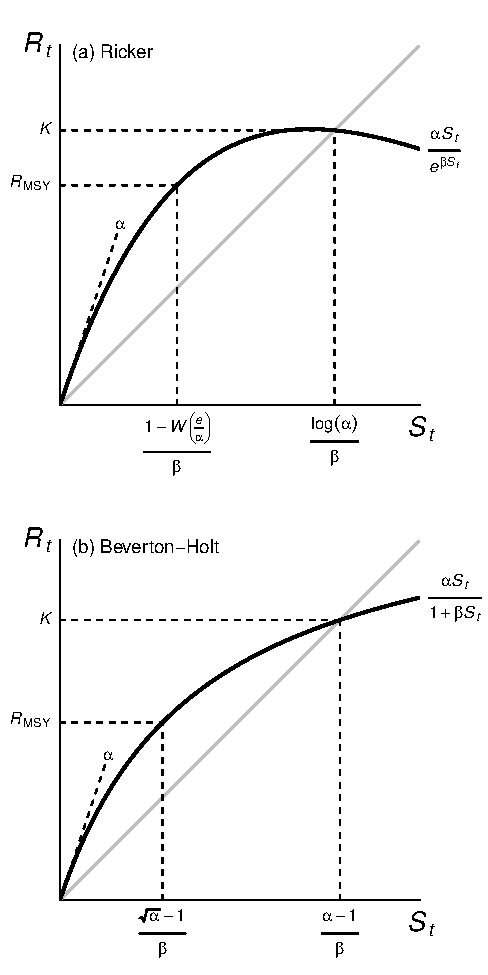
\includegraphics{App_3_Summarize_results_files/figure-latex/fig_1_model_forms-1} \end{center}

Figure 1: Deterministic forms of the (a) Ricker and (b) Beverton-Holt
models used in the analyses (thick lines), including equations for
carrying capacity (\(K\)) and the number of recruits corresponding to
the maximum sustained yield (\(R_{\text{MSY}}\)). The parameter
\(\alpha\) defines the slope at the origin, the constant \(e\) is
Euler's number, and \(W\) is the Lambert function (see Scheuerell 2016
for details). The gray line is where \(R_t = S_t\).

\hypertarget{fig-2---total-population-size}{%
\subsection{Fig 2 - Total population
size}\label{fig-2---total-population-size}}

Here is our estimate of the total run size (i.e., catch + escapement)
over time. The black points are the data, the blue line is the median
posterior estimate, and the shaded region is the 95\% credible interval.
Note that the y-axis is on a log scale.

\begin{Shaded}
\begin{Highlighting}[]
\NormalTok{clr }\OtherTok{\textless{}{-}} \FunctionTok{rgb}\NormalTok{(}\DecValTok{0}\NormalTok{, }\DecValTok{0}\NormalTok{, }\DecValTok{255}\NormalTok{, }\AttributeTok{alpha =} \DecValTok{50}\NormalTok{, }\AttributeTok{maxColorValue =} \DecValTok{255}\NormalTok{)}
\DocumentationTok{\#\# estimated spawner data for plotting}
\NormalTok{p\_dat }\OtherTok{\textless{}{-}}\NormalTok{ mod\_res[,}\FunctionTok{grep}\NormalTok{(}\StringTok{"Sp"}\NormalTok{, }\FunctionTok{colnames}\NormalTok{(mod\_res))]}
\NormalTok{p\_dat }\OtherTok{\textless{}{-}} \FunctionTok{apply}\NormalTok{(p\_dat, }\DecValTok{2}\NormalTok{, quantile, CI\_vec)}
\NormalTok{p\_dat }\OtherTok{\textless{}{-}}\NormalTok{ p\_dat }\SpecialCharTok{+} \FunctionTok{matrix}\NormalTok{(dat\_harv, }\FunctionTok{length}\NormalTok{(CI\_vec), n\_yrs, }\AttributeTok{byrow =} \ConstantTok{TRUE}\NormalTok{)}
\DocumentationTok{\#\# time seq}
\NormalTok{t\_idx\_f }\OtherTok{\textless{}{-}} \FunctionTok{seq}\NormalTok{(yr\_frst, }\AttributeTok{length.out =}\NormalTok{ n\_yrs)}
\DocumentationTok{\#\# plot}
\NormalTok{yp\_min }\OtherTok{\textless{}{-}} \FunctionTok{min}\NormalTok{(p\_dat)}
\NormalTok{yp\_max }\OtherTok{\textless{}{-}} \FunctionTok{max}\NormalTok{(p\_dat)}
\FunctionTok{par}\NormalTok{(}\AttributeTok{mai =} \FunctionTok{c}\NormalTok{(}\FloatTok{0.8}\NormalTok{,}\FloatTok{0.8}\NormalTok{,}\FloatTok{0.1}\NormalTok{,}\FloatTok{0.1}\NormalTok{), }\AttributeTok{omi =} \FunctionTok{c}\NormalTok{(}\FloatTok{0.5}\NormalTok{,}\FloatTok{0.2}\NormalTok{,}\FloatTok{0.6}\NormalTok{,}\FloatTok{0.2}\NormalTok{))}
\FunctionTok{plot}\NormalTok{(t\_idx\_f, p\_dat[}\DecValTok{3}\NormalTok{,], }\AttributeTok{ylim =} \FunctionTok{c}\NormalTok{(yp\_min,yp\_max), }\AttributeTok{type =} \StringTok{"n"}\NormalTok{,}
     \AttributeTok{log =} \StringTok{"y"}\NormalTok{, }\AttributeTok{xaxt =} \StringTok{"n"}\NormalTok{, }\AttributeTok{yaxt =} \StringTok{"n"}\NormalTok{, }\AttributeTok{bty =} \StringTok{"L"}\NormalTok{,}
     \AttributeTok{xlab =} \StringTok{"Year"}\NormalTok{, }\AttributeTok{ylab =} \StringTok{"Run size (catch + escapement)"}\NormalTok{, }\AttributeTok{main =} \StringTok{""}\NormalTok{, }\AttributeTok{cex.lab =} \FloatTok{1.2}\NormalTok{)}
\FunctionTok{polygon}\NormalTok{(}\FunctionTok{c}\NormalTok{(t\_idx\_f, }\FunctionTok{rev}\NormalTok{(t\_idx\_f)), }\FunctionTok{c}\NormalTok{(p\_dat[}\DecValTok{3}\NormalTok{,], }\FunctionTok{rev}\NormalTok{(p\_dat[}\DecValTok{1}\NormalTok{,])),}
        \AttributeTok{col =}\NormalTok{ clr, }\AttributeTok{border =} \ConstantTok{NA}\NormalTok{)}
\FunctionTok{lines}\NormalTok{(t\_idx\_f, p\_dat[}\DecValTok{2}\NormalTok{,], }\AttributeTok{col =} \StringTok{"blue3"}\NormalTok{, }\AttributeTok{lwd =} \DecValTok{2}\NormalTok{)}
\FunctionTok{points}\NormalTok{(t\_idx\_f, }\FunctionTok{exp}\NormalTok{(ln\_dat\_esc) }\SpecialCharTok{+}\NormalTok{ dat\_harv, }\AttributeTok{pch =} \DecValTok{16}\NormalTok{, }\AttributeTok{cex =} \DecValTok{1}\NormalTok{)}
\FunctionTok{axis}\NormalTok{(}\DecValTok{1}\NormalTok{, }\AttributeTok{at =} \FunctionTok{seq}\NormalTok{(}\DecValTok{1980}\NormalTok{, }\DecValTok{2015}\NormalTok{, }\DecValTok{5}\NormalTok{))}
\FunctionTok{axis}\NormalTok{(}\DecValTok{2}\NormalTok{, }\AttributeTok{at =} \FunctionTok{c}\NormalTok{(}\DecValTok{4000}\NormalTok{, }\DecValTok{8000}\NormalTok{, }\DecValTok{16000}\NormalTok{))}
\end{Highlighting}
\end{Shaded}

\begin{center}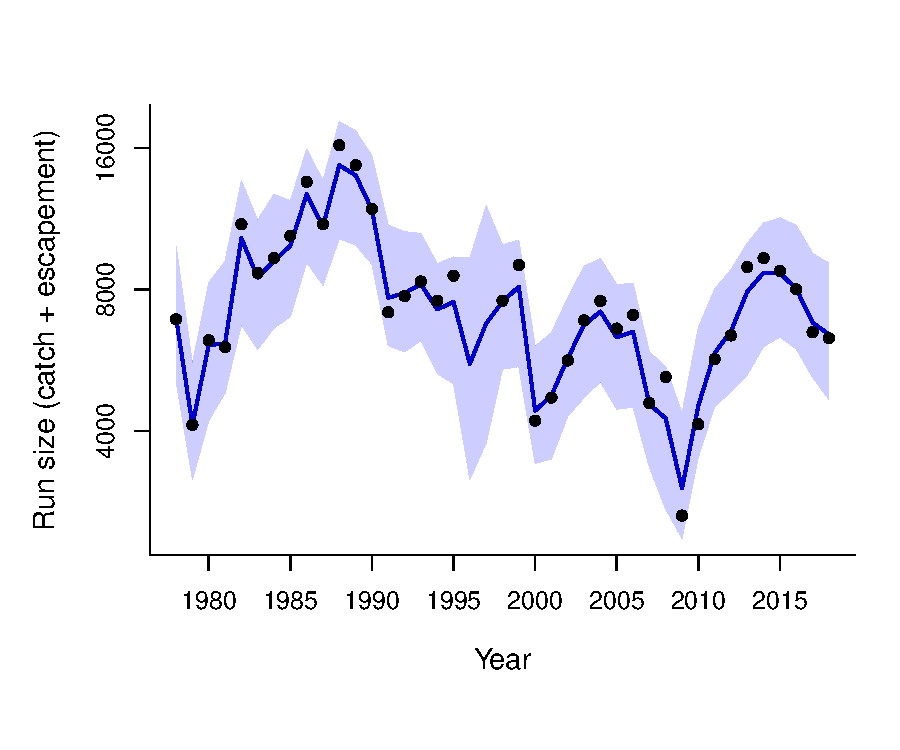
\includegraphics{App_3_Summarize_results_files/figure-latex/fig_2_run_size-1} \end{center}

Figure 2: Time series of the estimated total population size (catch plus
the adults that escaped to spawn). The observed data are the points; the
solid line is the median estimate and the shaded region indicates the
95\% credible interval.

\hypertarget{fig-3---spawner-recruit-relationship}{%
\subsection{Fig 3 - Spawner-recruit
relationship}\label{fig-3---spawner-recruit-relationship}}

Here is the relationship between spawner and subsequent recruits (a),
assuming mean values for all covariates. Gray lines show the median
relationship for each of the 41 years based on \(a_t\). Note that for
plotting purposes only in (b) and (c), the density in the largest bin
for each parameter contains counts for all values greater or equal to
that. Vertical arrows under the x-axes in (b) and (c) indicate the
2.5\textsuperscript{th}, 50\textsuperscript{th}, and
97.5\textsuperscript{th} percentiles.

\begin{Shaded}
\begin{Highlighting}[]
\FunctionTok{layout}\NormalTok{(}\FunctionTok{matrix}\NormalTok{(}\FunctionTok{c}\NormalTok{(}\DecValTok{1}\NormalTok{,}\DecValTok{1}\NormalTok{,}\DecValTok{2}\NormalTok{,}\DecValTok{3}\NormalTok{),}\DecValTok{2}\NormalTok{,}\DecValTok{2}\NormalTok{),}\FunctionTok{c}\NormalTok{(}\DecValTok{3}\NormalTok{,}\DecValTok{2}\NormalTok{),}\FunctionTok{c}\NormalTok{(}\DecValTok{1}\NormalTok{,}\DecValTok{1}\NormalTok{))}
\NormalTok{xoffSet }\OtherTok{\textless{}{-}} \FloatTok{0.05}
\NormalTok{yoffSet }\OtherTok{\textless{}{-}} \FloatTok{0.03}

\DocumentationTok{\#\# colors for plotting}
\NormalTok{clr }\OtherTok{\textless{}{-}} \FunctionTok{rgb}\NormalTok{(}\DecValTok{100}\NormalTok{, }\DecValTok{0}\NormalTok{, }\DecValTok{200}\NormalTok{,}
           \AttributeTok{alpha =} \FunctionTok{seq}\NormalTok{(}\DecValTok{200}\NormalTok{, }\DecValTok{100}\NormalTok{,}
                       \AttributeTok{length.out =}\NormalTok{ age\_max}\SpecialCharTok{{-}}\NormalTok{age\_min),}
           \AttributeTok{maxColorValue =} \DecValTok{255}\NormalTok{)}

\DocumentationTok{\#\# posterior of spawners}
\NormalTok{s\_dat }\OtherTok{\textless{}{-}}\NormalTok{ mod\_res[,}\FunctionTok{grep}\NormalTok{(}\StringTok{"Sp"}\NormalTok{, }\FunctionTok{colnames}\NormalTok{(mod\_res))]}
\NormalTok{s\_dat }\OtherTok{\textless{}{-}} \FunctionTok{apply}\NormalTok{(s\_dat, }\DecValTok{2}\NormalTok{, quantile, CI\_vec)}
\NormalTok{s\_dat }\OtherTok{\textless{}{-}}\NormalTok{ s\_dat[, }\DecValTok{1}\SpecialCharTok{:}\NormalTok{(n\_yrs}\SpecialCharTok{{-}}\NormalTok{age\_min)]}

\DocumentationTok{\#\# posterior of recruits}
\NormalTok{r\_dat }\OtherTok{\textless{}{-}}\NormalTok{ mod\_res[, }\FunctionTok{grep}\NormalTok{(}\StringTok{"tot\_ln\_Rec"}\NormalTok{, }\FunctionTok{colnames}\NormalTok{(mod\_res))]}
\NormalTok{r\_dat }\OtherTok{\textless{}{-}} \FunctionTok{exp}\NormalTok{(}\FunctionTok{apply}\NormalTok{(r\_dat, }\DecValTok{2}\NormalTok{, quantile, CI\_vec))}

\DocumentationTok{\#\# median values for a \& b}
\NormalTok{aa }\OtherTok{\textless{}{-}} \FunctionTok{apply}\NormalTok{(mod\_res[, }\FunctionTok{grep}\NormalTok{(}\StringTok{"ln\_BH\_a"}\NormalTok{, }\FunctionTok{colnames}\NormalTok{(mod\_res))], }\DecValTok{2}\NormalTok{, median)}
\NormalTok{bb }\OtherTok{\textless{}{-}} \FunctionTok{median}\NormalTok{(mod\_res[, }\StringTok{"beta"}\NormalTok{])}

\DocumentationTok{\#\# empty plot space for spawner{-}recruit relationships}
\NormalTok{dd }\OtherTok{\textless{}{-}} \DecValTok{3000}
\NormalTok{yM }\OtherTok{\textless{}{-}} \FunctionTok{around}\NormalTok{(}\FunctionTok{max}\NormalTok{(r\_dat), }\StringTok{"ceiling"}\NormalTok{, dd)}
\NormalTok{xM }\OtherTok{\textless{}{-}} \FunctionTok{around}\NormalTok{(}\FunctionTok{max}\NormalTok{(s\_dat), }\StringTok{"ceiling"}\NormalTok{, dd)}
\FunctionTok{par}\NormalTok{(}\AttributeTok{mai =} \FunctionTok{c}\NormalTok{(}\FloatTok{0.8}\NormalTok{,}\FloatTok{0.8}\NormalTok{,}\FloatTok{0.1}\NormalTok{,}\FloatTok{0.1}\NormalTok{), }\AttributeTok{omi =} \FunctionTok{c}\NormalTok{(}\DecValTok{0}\NormalTok{,}\DecValTok{0}\NormalTok{,}\DecValTok{0}\NormalTok{,}\DecValTok{0}\NormalTok{))}
\FunctionTok{plot}\NormalTok{(s\_dat[}\DecValTok{2}\NormalTok{,], r\_dat[}\DecValTok{2}\NormalTok{,], }\AttributeTok{xlim =} \FunctionTok{c}\NormalTok{(}\DecValTok{0}\NormalTok{,xM), }\AttributeTok{ylim =} \FunctionTok{c}\NormalTok{(}\DecValTok{0}\NormalTok{,yM), }\AttributeTok{type =} \StringTok{"n"}\NormalTok{,}
     \AttributeTok{xaxs =} \StringTok{"i"}\NormalTok{, }\AttributeTok{yaxs =} \StringTok{"i"}\NormalTok{, }\AttributeTok{cex.lab =} \FloatTok{1.2}\NormalTok{,}
     \AttributeTok{xlab =} \FunctionTok{expression}\NormalTok{(Spawners}\SpecialCharTok{\textasciitilde{}}\NormalTok{(}\DecValTok{10}\SpecialCharTok{\^{}}\DecValTok{3}\NormalTok{)),}
     \AttributeTok{ylab =} \FunctionTok{expression}\NormalTok{(Recruits}\SpecialCharTok{\textasciitilde{}}\NormalTok{(}\DecValTok{10}\SpecialCharTok{\^{}}\DecValTok{3}\NormalTok{)),}
     \AttributeTok{xaxt =} \StringTok{"n"}\NormalTok{, }\AttributeTok{yaxt =} \StringTok{"n"}\NormalTok{, }\AttributeTok{bty=}\StringTok{"L"}\NormalTok{)}
\FunctionTok{axis}\NormalTok{(}\DecValTok{1}\NormalTok{, }\AttributeTok{at =} \FunctionTok{seq}\NormalTok{(}\DecValTok{0}\NormalTok{,xM,dd}\SpecialCharTok{*}\DecValTok{2}\NormalTok{), }\AttributeTok{labels =} \FunctionTok{seq}\NormalTok{(}\DecValTok{0}\NormalTok{,xM,dd}\SpecialCharTok{*}\DecValTok{2}\NormalTok{)}\SpecialCharTok{/}\DecValTok{1000}\NormalTok{)}
\FunctionTok{axis}\NormalTok{(}\DecValTok{2}\NormalTok{, }\AttributeTok{at =} \FunctionTok{seq}\NormalTok{(}\DecValTok{0}\NormalTok{,yM,dd}\SpecialCharTok{*}\DecValTok{2}\NormalTok{), }\AttributeTok{labels =} \FunctionTok{seq}\NormalTok{(}\DecValTok{0}\NormalTok{,yM,dd}\SpecialCharTok{*}\DecValTok{2}\NormalTok{)}\SpecialCharTok{/}\DecValTok{1000}\NormalTok{, }\AttributeTok{las=}\DecValTok{1}\NormalTok{)}
\ControlFlowTok{for}\NormalTok{(i }\ControlFlowTok{in} \DecValTok{1}\SpecialCharTok{:}\FunctionTok{length}\NormalTok{(aa)) \{}
  \FunctionTok{lines}\NormalTok{(}\FunctionTok{exp}\NormalTok{(aa[i]) }\SpecialCharTok{*} \FunctionTok{seq}\NormalTok{(}\DecValTok{0}\NormalTok{,xM) }\SpecialCharTok{/}\NormalTok{ (}\DecValTok{1} \SpecialCharTok{+}\NormalTok{ bb }\SpecialCharTok{*} \FunctionTok{seq}\NormalTok{(}\DecValTok{0}\NormalTok{,xM)),}
        \AttributeTok{col =} \StringTok{"darkgray"}\NormalTok{)}
\NormalTok{\}}
\FunctionTok{abline}\NormalTok{(}\AttributeTok{a =} \DecValTok{0}\NormalTok{,}\AttributeTok{b =} \DecValTok{1}\NormalTok{,}\AttributeTok{lty =} \StringTok{"dashed"}\NormalTok{)}

\DocumentationTok{\#\# add S{-}R estimates and medians}
\NormalTok{nCB }\OtherTok{\textless{}{-}}\NormalTok{ n\_yrs}\SpecialCharTok{{-}}\NormalTok{age\_max}
\DocumentationTok{\#\# years with complete returns}
\FunctionTok{points}\NormalTok{(s\_dat[}\DecValTok{2}\NormalTok{, }\DecValTok{1}\SpecialCharTok{:}\NormalTok{nCB], r\_dat[}\DecValTok{2}\NormalTok{, }\DecValTok{1}\SpecialCharTok{:}\NormalTok{nCB],}
       \AttributeTok{xlim =} \FunctionTok{c}\NormalTok{(}\DecValTok{0}\NormalTok{,xM), }\AttributeTok{ylim =} \FunctionTok{c}\NormalTok{(}\DecValTok{0}\NormalTok{,yM),}
       \AttributeTok{pch =} \DecValTok{16}\NormalTok{, }\AttributeTok{col =} \StringTok{"blue3"}\NormalTok{)}
\FunctionTok{segments}\NormalTok{(s\_dat[}\DecValTok{2}\NormalTok{, }\DecValTok{1}\SpecialCharTok{:}\NormalTok{nCB], r\_dat[}\DecValTok{1}\NormalTok{, }\DecValTok{1}\SpecialCharTok{:}\NormalTok{nCB],}
\NormalTok{         s\_dat[}\DecValTok{2}\NormalTok{, }\DecValTok{1}\SpecialCharTok{:}\NormalTok{nCB], r\_dat[}\DecValTok{3}\NormalTok{, }\DecValTok{1}\SpecialCharTok{:}\NormalTok{nCB],}
         \AttributeTok{col =} \StringTok{"blue3"}\NormalTok{)}
\FunctionTok{segments}\NormalTok{(s\_dat[}\DecValTok{1}\NormalTok{, }\DecValTok{1}\SpecialCharTok{:}\NormalTok{nCB], r\_dat[}\DecValTok{2}\NormalTok{, }\DecValTok{1}\SpecialCharTok{:}\NormalTok{nCB],}
\NormalTok{         s\_dat[}\DecValTok{3}\NormalTok{, }\DecValTok{1}\SpecialCharTok{:}\NormalTok{nCB], r\_dat[}\DecValTok{2}\NormalTok{, }\DecValTok{1}\SpecialCharTok{:}\NormalTok{nCB],}
         \AttributeTok{col =} \StringTok{"blue3"}\NormalTok{)}
\NormalTok{nTB }\OtherTok{\textless{}{-}} \FunctionTok{dim}\NormalTok{(s\_dat)[}\DecValTok{2}\NormalTok{]}
\DocumentationTok{\#\# years with incomplete returns}
\FunctionTok{segments}\NormalTok{(s\_dat[}\DecValTok{2}\NormalTok{, (nCB}\SpecialCharTok{+}\DecValTok{1}\NormalTok{)}\SpecialCharTok{:}\NormalTok{nTB], r\_dat[}\DecValTok{1}\NormalTok{, (nCB}\SpecialCharTok{+}\DecValTok{1}\NormalTok{)}\SpecialCharTok{:}\NormalTok{nTB],}
\NormalTok{         s\_dat[}\DecValTok{2}\NormalTok{, (nCB}\SpecialCharTok{+}\DecValTok{1}\NormalTok{)}\SpecialCharTok{:}\NormalTok{nTB], r\_dat[}\DecValTok{3}\NormalTok{, (nCB}\SpecialCharTok{+}\DecValTok{1}\NormalTok{)}\SpecialCharTok{:}\NormalTok{nTB],}
         \AttributeTok{col =}\NormalTok{ clr)}
\FunctionTok{segments}\NormalTok{(s\_dat[}\DecValTok{1}\NormalTok{, (nCB}\SpecialCharTok{+}\DecValTok{1}\NormalTok{)}\SpecialCharTok{:}\NormalTok{nTB], r\_dat[}\DecValTok{2}\NormalTok{, (nCB}\SpecialCharTok{+}\DecValTok{1}\NormalTok{)}\SpecialCharTok{:}\NormalTok{nTB],}
\NormalTok{         s\_dat[}\DecValTok{3}\NormalTok{, (nCB}\SpecialCharTok{+}\DecValTok{1}\NormalTok{)}\SpecialCharTok{:}\NormalTok{nTB], r\_dat[}\DecValTok{2}\NormalTok{, (nCB}\SpecialCharTok{+}\DecValTok{1}\NormalTok{)}\SpecialCharTok{:}\NormalTok{nTB],}
         \AttributeTok{col =}\NormalTok{ clr)}
\FunctionTok{points}\NormalTok{(s\_dat[}\DecValTok{2}\NormalTok{, (nCB}\SpecialCharTok{+}\DecValTok{1}\NormalTok{)}\SpecialCharTok{:}\NormalTok{nTB],r\_dat[}\DecValTok{2}\NormalTok{, (nCB}\SpecialCharTok{+}\DecValTok{1}\NormalTok{)}\SpecialCharTok{:}\NormalTok{nTB],}
       \AttributeTok{xlim =} \FunctionTok{c}\NormalTok{(}\DecValTok{0}\NormalTok{,xM), }\AttributeTok{ylim =} \FunctionTok{c}\NormalTok{(}\DecValTok{0}\NormalTok{,yM),}
       \AttributeTok{pch =} \DecValTok{16}\NormalTok{, }\AttributeTok{col =}\NormalTok{ clr)}
\FunctionTok{text}\NormalTok{(}\AttributeTok{x =} \FunctionTok{par}\NormalTok{()}\SpecialCharTok{$}\NormalTok{usr[}\DecValTok{1}\NormalTok{] }\SpecialCharTok{+} \FunctionTok{diff}\NormalTok{(}\FunctionTok{par}\NormalTok{()}\SpecialCharTok{$}\NormalTok{usr[}\DecValTok{1}\SpecialCharTok{:}\DecValTok{2}\NormalTok{]) }\SpecialCharTok{*}\NormalTok{ xoffSet,}
     \AttributeTok{y =} \FunctionTok{par}\NormalTok{()}\SpecialCharTok{$}\NormalTok{usr[}\DecValTok{4}\NormalTok{] }\SpecialCharTok{{-}} \FunctionTok{diff}\NormalTok{(}\FunctionTok{par}\NormalTok{()}\SpecialCharTok{$}\NormalTok{usr[}\DecValTok{3}\SpecialCharTok{:}\DecValTok{4}\NormalTok{]) }\SpecialCharTok{*}\NormalTok{ yoffSet,}
     \StringTok{"(a)"}\NormalTok{)}

\DocumentationTok{\#\# posterior for alpha}
\NormalTok{clr }\OtherTok{\textless{}{-}} \FunctionTok{rgb}\NormalTok{(}\DecValTok{0}\NormalTok{, }\DecValTok{0}\NormalTok{, }\DecValTok{255}\NormalTok{, }\AttributeTok{alpha =} \DecValTok{50}\NormalTok{, }\AttributeTok{maxColorValue =} \DecValTok{255}\NormalTok{)}
\NormalTok{a\_thresh }\OtherTok{\textless{}{-}} \DecValTok{59}
\FunctionTok{par}\NormalTok{(}\AttributeTok{mai =} \FunctionTok{c}\NormalTok{(}\FloatTok{0.8}\NormalTok{,}\FloatTok{0.4}\NormalTok{,}\FloatTok{0.3}\NormalTok{,}\FloatTok{0.1}\NormalTok{))}
\DocumentationTok{\#\# B{-}H alpha}
\NormalTok{R\_alpha\_est }\OtherTok{\textless{}{-}}\NormalTok{ mod\_res[, }\StringTok{"alpha"}\NormalTok{]}
\NormalTok{alphaCI }\OtherTok{\textless{}{-}} \FunctionTok{quantile}\NormalTok{(R\_alpha\_est, CI\_vec)}
\NormalTok{R\_alpha\_est[R\_alpha\_est }\SpecialCharTok{\textgreater{}}\NormalTok{ a\_thresh] }\OtherTok{\textless{}{-}}\NormalTok{ a\_thresh}
\FunctionTok{hist}\NormalTok{(R\_alpha\_est, }\AttributeTok{freq =} \ConstantTok{FALSE}\NormalTok{, }\AttributeTok{breaks =} \FunctionTok{seq}\NormalTok{(}\DecValTok{0}\NormalTok{, a\_thresh}\SpecialCharTok{+}\DecValTok{1}\NormalTok{, }\DecValTok{2}\NormalTok{),}
     \AttributeTok{col =}\NormalTok{ clr, }\AttributeTok{border =} \StringTok{"blue3"}\NormalTok{,}
     \AttributeTok{xlab =} \StringTok{""}\NormalTok{, }\AttributeTok{ylab =} \StringTok{""}\NormalTok{, }\AttributeTok{main =} \StringTok{""}\NormalTok{, }\AttributeTok{cex.lab =} \FloatTok{1.2}\NormalTok{, }\AttributeTok{yaxt =} \StringTok{"n"}\NormalTok{)}
\NormalTok{aHt }\OtherTok{\textless{}{-}}\NormalTok{ (}\FunctionTok{par}\NormalTok{()}\SpecialCharTok{$}\NormalTok{usr[}\DecValTok{4}\NormalTok{]}\SpecialCharTok{{-}}\FunctionTok{par}\NormalTok{()}\SpecialCharTok{$}\NormalTok{usr[}\DecValTok{3}\NormalTok{])}\SpecialCharTok{/}\DecValTok{12}
\FunctionTok{arrows}\NormalTok{(alphaCI, }\FunctionTok{par}\NormalTok{()}\SpecialCharTok{$}\NormalTok{usr[}\DecValTok{3}\NormalTok{], alphaCI,}\FunctionTok{par}\NormalTok{()}\SpecialCharTok{$}\NormalTok{usr[}\DecValTok{3}\NormalTok{]}\SpecialCharTok{{-}}\NormalTok{aHt,}
       \AttributeTok{code =} \DecValTok{1}\NormalTok{, }\AttributeTok{length =} \FloatTok{0.05}\NormalTok{, }\AttributeTok{xpd =} \ConstantTok{NA}\NormalTok{, }\AttributeTok{col =} \StringTok{"blue3"}\NormalTok{, }\AttributeTok{lwd =} \FloatTok{1.5}\NormalTok{)}
\FunctionTok{mtext}\NormalTok{(}\FunctionTok{expression}\NormalTok{(Instrinsic}\SpecialCharTok{\textasciitilde{}}\NormalTok{productivity}\SpecialCharTok{\textasciitilde{}}\NormalTok{(alpha)), }\DecValTok{1}\NormalTok{, }\AttributeTok{line =} \DecValTok{3}\NormalTok{, }\AttributeTok{cex =} \DecValTok{1}\NormalTok{)}
\FunctionTok{text}\NormalTok{(}\AttributeTok{x =} \FunctionTok{par}\NormalTok{()}\SpecialCharTok{$}\NormalTok{usr[}\DecValTok{1}\NormalTok{],}
     \AttributeTok{y =} \FunctionTok{par}\NormalTok{()}\SpecialCharTok{$}\NormalTok{usr[}\DecValTok{4}\NormalTok{] }\SpecialCharTok{*} \FloatTok{1.05}\NormalTok{,}
     \StringTok{"(b)"}\NormalTok{, }\AttributeTok{xpd=}\ConstantTok{NA}\NormalTok{)}

\DocumentationTok{\#\# posterior for K}
\FunctionTok{par}\NormalTok{(}\AttributeTok{mai =} \FunctionTok{c}\NormalTok{(}\FloatTok{0.8}\NormalTok{,}\FloatTok{0.4}\NormalTok{,}\FloatTok{0.3}\NormalTok{,}\FloatTok{0.1}\NormalTok{))}
\NormalTok{aa }\OtherTok{\textless{}{-}}\NormalTok{ mod\_res[, }\StringTok{"alpha"}\NormalTok{]}
\NormalTok{bb }\OtherTok{\textless{}{-}}\NormalTok{ mod\_res[, }\StringTok{"beta"}\NormalTok{]}
\DocumentationTok{\#\# K in 1000s}
\NormalTok{R\_b\_est }\OtherTok{\textless{}{-}}\NormalTok{ (aa}\DecValTok{{-}1}\NormalTok{) }\SpecialCharTok{/}\NormalTok{ bb }\SpecialCharTok{/} \DecValTok{1000}
\NormalTok{R\_b\_est }\OtherTok{\textless{}{-}}\NormalTok{ R\_b\_est[R\_b\_est }\SpecialCharTok{\textgreater{}} \DecValTok{0}\NormalTok{]}
\NormalTok{R\_b\_CI }\OtherTok{\textless{}{-}} \FunctionTok{quantile}\NormalTok{(R\_b\_est, CI\_vec)}
\DocumentationTok{\#\# pile into last ban for plotting}
\NormalTok{R\_b\_est[R\_b\_est }\SpecialCharTok{\textgreater{}} \DecValTok{13}\NormalTok{] }\OtherTok{\textless{}{-}} \DecValTok{13}
\NormalTok{brks }\OtherTok{\textless{}{-}} \FunctionTok{seq}\NormalTok{(}\FunctionTok{around}\NormalTok{(}\FunctionTok{min}\NormalTok{(R\_b\_est), }\StringTok{"floor"}\NormalTok{),}
            \FunctionTok{around}\NormalTok{(}\FunctionTok{max}\NormalTok{(R\_b\_est), }\StringTok{"ceiling"}\NormalTok{),}
            \AttributeTok{length.out =} \FunctionTok{length}\NormalTok{(}\FunctionTok{seq}\NormalTok{(}\DecValTok{0}\NormalTok{, a\_thresh, }\DecValTok{2}\NormalTok{)))}
\FunctionTok{hist}\NormalTok{(R\_b\_est, }\AttributeTok{freq =} \ConstantTok{FALSE}\NormalTok{, }\AttributeTok{breaks =}\NormalTok{ brks, }\AttributeTok{col =}\NormalTok{ clr, }\AttributeTok{border =} \StringTok{"blue3"}\NormalTok{,}
     \AttributeTok{xlab =} \StringTok{""}\NormalTok{, }\AttributeTok{xaxt =} \StringTok{"n"}\NormalTok{, }\AttributeTok{yaxt =} \StringTok{"n"}\NormalTok{,}
     \AttributeTok{main =} \StringTok{""}\NormalTok{, }\AttributeTok{ylab =} \StringTok{""}\NormalTok{, }\AttributeTok{cex.lab =} \FloatTok{1.2}\NormalTok{)}
\FunctionTok{axis}\NormalTok{(}\DecValTok{1}\NormalTok{, }\AttributeTok{at =} \FunctionTok{seq}\NormalTok{(}\FunctionTok{around}\NormalTok{(}\FunctionTok{min}\NormalTok{(R\_b\_est), }\StringTok{"floor"}\NormalTok{),}
                 \FunctionTok{around}\NormalTok{(}\FunctionTok{max}\NormalTok{(R\_b\_est), }\StringTok{"ceiling"}\NormalTok{),}
                 \DecValTok{2}\NormalTok{))}
\NormalTok{aHt }\OtherTok{\textless{}{-}}\NormalTok{ (}\FunctionTok{par}\NormalTok{()}\SpecialCharTok{$}\NormalTok{usr[}\DecValTok{4}\NormalTok{] }\SpecialCharTok{{-}} \FunctionTok{par}\NormalTok{()}\SpecialCharTok{$}\NormalTok{usr[}\DecValTok{3}\NormalTok{]) }\SpecialCharTok{/} \DecValTok{12}
\FunctionTok{arrows}\NormalTok{(R\_b\_CI, }\FunctionTok{par}\NormalTok{()}\SpecialCharTok{$}\NormalTok{usr[}\DecValTok{3}\NormalTok{], R\_b\_CI,}\FunctionTok{par}\NormalTok{()}\SpecialCharTok{$}\NormalTok{usr[}\DecValTok{3}\NormalTok{]}\SpecialCharTok{{-}}\NormalTok{aHt,}
       \AttributeTok{code =} \DecValTok{1}\NormalTok{, }\AttributeTok{length =} \FloatTok{0.05}\NormalTok{, }\AttributeTok{xpd =} \ConstantTok{NA}\NormalTok{, }\AttributeTok{col =} \StringTok{"blue3"}\NormalTok{, }\AttributeTok{lwd =} \FloatTok{1.5}\NormalTok{)}
\FunctionTok{mtext}\NormalTok{(}\FunctionTok{expression}\NormalTok{(}\FunctionTok{paste}\NormalTok{(}\StringTok{"Carrying capacity ("}\NormalTok{,}\FunctionTok{italic}\NormalTok{(K),}\StringTok{", "}\NormalTok{,}\DecValTok{10}\SpecialCharTok{\^{}}\DecValTok{3}\NormalTok{,}\StringTok{")"}\NormalTok{)),}
      \AttributeTok{side =} \DecValTok{1}\NormalTok{, }\AttributeTok{line =} \DecValTok{3}\NormalTok{, }\AttributeTok{cex =} \DecValTok{1}\NormalTok{)}
\FunctionTok{text}\NormalTok{(}\AttributeTok{x =} \FunctionTok{par}\NormalTok{()}\SpecialCharTok{$}\NormalTok{usr[}\DecValTok{1}\NormalTok{], }
     \AttributeTok{y =} \FunctionTok{par}\NormalTok{()}\SpecialCharTok{$}\NormalTok{usr[}\DecValTok{4}\NormalTok{] }\SpecialCharTok{*} \FloatTok{1.05}\NormalTok{,}
     \StringTok{"(c)"}\NormalTok{, }\AttributeTok{xpd=}\ConstantTok{NA}\NormalTok{)}
\end{Highlighting}
\end{Shaded}

\begin{center}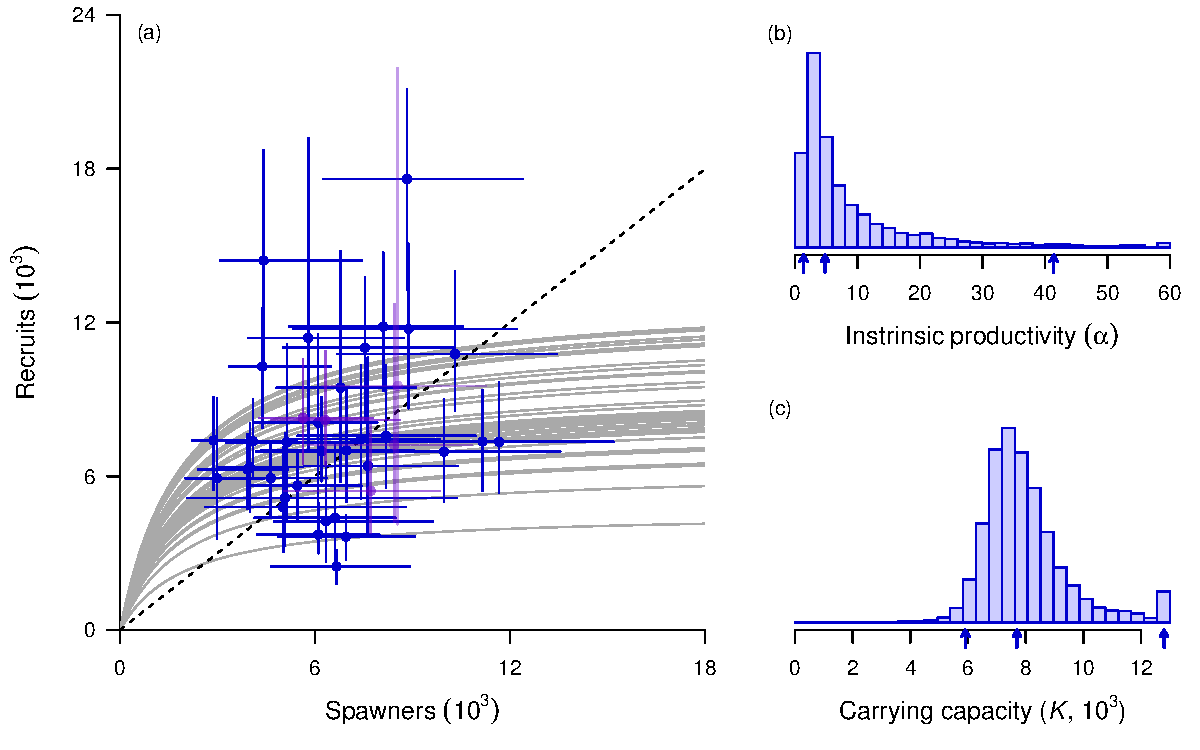
\includegraphics{App_3_Summarize_results_files/figure-latex/fig_3_S-R-1} \end{center}

Figure 3: Relationship between the number of spawning adults and their
subsequent surviving offspring (recruits), assuming mean values for all
covariates (a); and the estimated posterior distributions for the
intrinsic productivity (b) and carrying capacity (c). Points in (a) are
medians of the posterior estimates; error bars indicate the 95\%
credible intervals. Blue points are for estimates with complete broods;
purple points are for the most recent years with incomplete broods. Gray
lines show the median relationship for each of the 41 years in the time
series based on annual model estimates of productivity. Note that for
plotting purposes only in (b) and (c), the density in the largest bin
for each parameter contains counts for all values greater than or equal
to it. Vertical arrows under the x-axes in (b) and (c) indicate the
2.5\(^\text{th}\), 50\(^\text{th}\), and 97.5\(^\text{th}\) percentiles.

\hypertarget{fig-4---covariate-effects}{%
\subsection{Fig 4 - Covariate effects}\label{fig-4---covariate-effects}}

Here are time series plots of the covariates (a-c) and histograms of
their effects on productivity (d-f).

\begin{Shaded}
\begin{Highlighting}[]
\NormalTok{clr }\OtherTok{\textless{}{-}} \FunctionTok{rgb}\NormalTok{(}\DecValTok{0}\NormalTok{, }\DecValTok{0}\NormalTok{, }\DecValTok{255}\NormalTok{, }\AttributeTok{alpha =} \DecValTok{50}\NormalTok{, }\AttributeTok{maxColorValue =} \DecValTok{255}\NormalTok{)}
\NormalTok{xoffSet }\OtherTok{\textless{}{-}} \FloatTok{0.04}
\NormalTok{yoffSet }\OtherTok{\textless{}{-}} \FloatTok{0.03}

\FunctionTok{par}\NormalTok{(}\AttributeTok{mfrow=}\FunctionTok{c}\NormalTok{(n\_cov,}\DecValTok{2}\NormalTok{), }\AttributeTok{mai=}\FunctionTok{c}\NormalTok{(}\FloatTok{0.4}\NormalTok{,}\FloatTok{0.2}\NormalTok{,}\FloatTok{0.1}\NormalTok{,}\FloatTok{0.1}\NormalTok{), }\AttributeTok{omi=}\FunctionTok{c}\NormalTok{(}\FloatTok{0.2}\NormalTok{,}\FloatTok{0.5}\NormalTok{,}\DecValTok{0}\NormalTok{,}\DecValTok{0}\NormalTok{))}

\NormalTok{c\_est }\OtherTok{\textless{}{-}}\NormalTok{ mod\_res[,}\FunctionTok{grep}\NormalTok{(}\StringTok{"gamma"}\NormalTok{, }\FunctionTok{colnames}\NormalTok{(mod\_res))]}
\NormalTok{ylN }\OtherTok{\textless{}{-}} \FunctionTok{floor}\NormalTok{(}\FunctionTok{min}\NormalTok{(c\_est)}\SpecialCharTok{*}\DecValTok{10}\NormalTok{)}\SpecialCharTok{/}\DecValTok{10}
\NormalTok{ylM }\OtherTok{\textless{}{-}} \FunctionTok{ceiling}\NormalTok{(}\FunctionTok{max}\NormalTok{(c\_est)}\SpecialCharTok{*}\DecValTok{10}\NormalTok{)}\SpecialCharTok{/}\DecValTok{10}
\NormalTok{brks }\OtherTok{\textless{}{-}} \FunctionTok{seq}\NormalTok{(ylN,ylM,}\AttributeTok{length.out=}\FunctionTok{diff}\NormalTok{(}\FunctionTok{c}\NormalTok{(ylN,ylM))}\SpecialCharTok{*}\DecValTok{40}\SpecialCharTok{+}\DecValTok{1}\NormalTok{)}
\NormalTok{t\_idx }\OtherTok{\textless{}{-}} \FunctionTok{seq}\NormalTok{(yr\_frst,}\AttributeTok{length.out=}\NormalTok{n\_yrs}\SpecialCharTok{{-}}\NormalTok{age\_min)}
\NormalTok{dat\_cvrs }\OtherTok{\textless{}{-}} \FunctionTok{as.matrix}\NormalTok{(dat\_cvrs[}\FunctionTok{seq}\NormalTok{(}\FunctionTok{length}\NormalTok{(t\_idx)),])}

\ControlFlowTok{for}\NormalTok{(i }\ControlFlowTok{in} \DecValTok{1}\SpecialCharTok{:}\NormalTok{n\_cov) \{}
  \ControlFlowTok{if}\NormalTok{(i}\SpecialCharTok{==}\DecValTok{4}\NormalTok{) \{}
\NormalTok{    dat\_cvrs[,i}\SpecialCharTok{+}\DecValTok{1}\NormalTok{] }\OtherTok{\textless{}{-}}\NormalTok{ dat\_cvrs[,i}\SpecialCharTok{+}\DecValTok{1}\NormalTok{]}\SpecialCharTok{/}\DecValTok{1000}
\NormalTok{  \}}
  \DocumentationTok{\#\# plot covar ts}
  \FunctionTok{plot}\NormalTok{(dat\_cvrs[, }\StringTok{"year"}\NormalTok{], dat\_cvrs[, i}\SpecialCharTok{+}\DecValTok{1}\NormalTok{],}
       \AttributeTok{pch =} \DecValTok{16}\NormalTok{, }\AttributeTok{col =} \StringTok{"blue3"}\NormalTok{, }\AttributeTok{type =} \StringTok{"o"}\NormalTok{,}
       \AttributeTok{xlab =} \StringTok{""}\NormalTok{, }\AttributeTok{ylab =} \StringTok{""}\NormalTok{, }\AttributeTok{main =} \StringTok{""}\NormalTok{, }\AttributeTok{bty =} \StringTok{"L"}\NormalTok{,}
       \AttributeTok{cex.axis =} \FloatTok{1.2}\NormalTok{)}
  \FunctionTok{text}\NormalTok{(}\AttributeTok{x =} \FunctionTok{par}\NormalTok{()}\SpecialCharTok{$}\NormalTok{usr[}\DecValTok{1}\NormalTok{] }\SpecialCharTok{+} \FunctionTok{diff}\NormalTok{(}\FunctionTok{par}\NormalTok{()}\SpecialCharTok{$}\NormalTok{usr[}\DecValTok{1}\SpecialCharTok{:}\DecValTok{2}\NormalTok{]) }\SpecialCharTok{*}\NormalTok{ xoffSet,}
       \AttributeTok{y =} \FunctionTok{par}\NormalTok{()}\SpecialCharTok{$}\NormalTok{usr[}\DecValTok{4}\NormalTok{] }\SpecialCharTok{{-}} \FunctionTok{diff}\NormalTok{(}\FunctionTok{par}\NormalTok{()}\SpecialCharTok{$}\NormalTok{usr[}\DecValTok{3}\SpecialCharTok{:}\DecValTok{4}\NormalTok{]) }\SpecialCharTok{*}\NormalTok{ yoffSet,}
       \FunctionTok{paste0}\NormalTok{(}\StringTok{"("}\NormalTok{,letters[i],}\StringTok{")"}\NormalTok{),}
       \AttributeTok{cex =} \FloatTok{1.2}\NormalTok{)}
  \FunctionTok{mtext}\NormalTok{(}\AttributeTok{side =} \DecValTok{2}\NormalTok{, cov\_names[i], }\AttributeTok{line =} \DecValTok{3}\NormalTok{, }\AttributeTok{cex =} \FloatTok{1.2}\NormalTok{)}
  \ControlFlowTok{if}\NormalTok{(i }\SpecialCharTok{==}\NormalTok{ n\_cov) \{}
    \FunctionTok{mtext}\NormalTok{(}\AttributeTok{side =} \DecValTok{1}\NormalTok{, }\StringTok{"Brood year"}\NormalTok{, }\AttributeTok{line =} \DecValTok{3}\NormalTok{)}
\NormalTok{  \}}
  \DocumentationTok{\#\# plot covar effect}
  \FunctionTok{hist}\NormalTok{(c\_est[,i],}
       \AttributeTok{freq =} \ConstantTok{FALSE}\NormalTok{, }\AttributeTok{breaks =}\NormalTok{ brks, }\AttributeTok{col =}\NormalTok{ clr, }\AttributeTok{border =}\StringTok{" blue3"}\NormalTok{,}
       \AttributeTok{xlab =} \StringTok{""}\NormalTok{, }\AttributeTok{yaxt =} \StringTok{"n"}\NormalTok{, }\AttributeTok{main =} \StringTok{""}\NormalTok{, }\AttributeTok{ylab =} \StringTok{""}\NormalTok{, }\AttributeTok{cex.axis =} \FloatTok{1.2}\NormalTok{)}
\NormalTok{  c\_CI }\OtherTok{\textless{}{-}} \FunctionTok{quantile}\NormalTok{(c\_est[,i],CI\_vec)}
\NormalTok{  aHt }\OtherTok{\textless{}{-}}\NormalTok{ (}\FunctionTok{par}\NormalTok{()}\SpecialCharTok{$}\NormalTok{usr[}\DecValTok{4}\NormalTok{]}\SpecialCharTok{{-}}\FunctionTok{par}\NormalTok{()}\SpecialCharTok{$}\NormalTok{usr[}\DecValTok{3}\NormalTok{])}\SpecialCharTok{/}\DecValTok{20}
  \FunctionTok{arrows}\NormalTok{(c\_CI, }\FunctionTok{par}\NormalTok{()}\SpecialCharTok{$}\NormalTok{usr[}\DecValTok{3}\NormalTok{]}\SpecialCharTok{{-}}\FloatTok{0.005}\NormalTok{, c\_CI, }\FunctionTok{par}\NormalTok{()}\SpecialCharTok{$}\NormalTok{usr[}\DecValTok{3}\NormalTok{] }\SpecialCharTok{{-}}\NormalTok{ aHt,}
         \AttributeTok{code =} \DecValTok{1}\NormalTok{,}\AttributeTok{length =} \FloatTok{0.05}\NormalTok{, }\AttributeTok{xpd =} \ConstantTok{NA}\NormalTok{, }\AttributeTok{col =} \StringTok{"blue3"}\NormalTok{, }\AttributeTok{lwd =} \FloatTok{1.5}\NormalTok{)}
  \FunctionTok{abline}\NormalTok{(}\AttributeTok{v =} \DecValTok{0}\NormalTok{, }\AttributeTok{lty =} \StringTok{"dashed"}\NormalTok{)}
  \FunctionTok{text}\NormalTok{(}\AttributeTok{x =} \FunctionTok{par}\NormalTok{()}\SpecialCharTok{$}\NormalTok{usr[}\DecValTok{1}\NormalTok{] }\SpecialCharTok{+} \FunctionTok{diff}\NormalTok{(}\FunctionTok{par}\NormalTok{()}\SpecialCharTok{$}\NormalTok{usr[}\DecValTok{1}\SpecialCharTok{:}\DecValTok{2}\NormalTok{]) }\SpecialCharTok{*}\NormalTok{ xoffSet,}
       \AttributeTok{y =} \FunctionTok{par}\NormalTok{()}\SpecialCharTok{$}\NormalTok{usr[}\DecValTok{4}\NormalTok{] }\SpecialCharTok{{-}} \FunctionTok{diff}\NormalTok{(}\FunctionTok{par}\NormalTok{()}\SpecialCharTok{$}\NormalTok{usr[}\DecValTok{3}\SpecialCharTok{:}\DecValTok{4}\NormalTok{]) }\SpecialCharTok{*}\NormalTok{ yoffSet,}
       \FunctionTok{paste0}\NormalTok{(}\StringTok{"("}\NormalTok{,letters[i}\SpecialCharTok{+}\NormalTok{n\_cov],}\StringTok{")"}\NormalTok{),}
       \AttributeTok{cex =} \FloatTok{1.2}\NormalTok{)}
  \ControlFlowTok{if}\NormalTok{(i }\SpecialCharTok{==}\NormalTok{ n\_cov) \{ }\FunctionTok{mtext}\NormalTok{(}\AttributeTok{side =} \DecValTok{1}\NormalTok{,}\StringTok{"Effect size"}\NormalTok{, }\AttributeTok{line =} \DecValTok{3}\NormalTok{) \}}
\NormalTok{\}}
\end{Highlighting}
\end{Shaded}

\begin{center}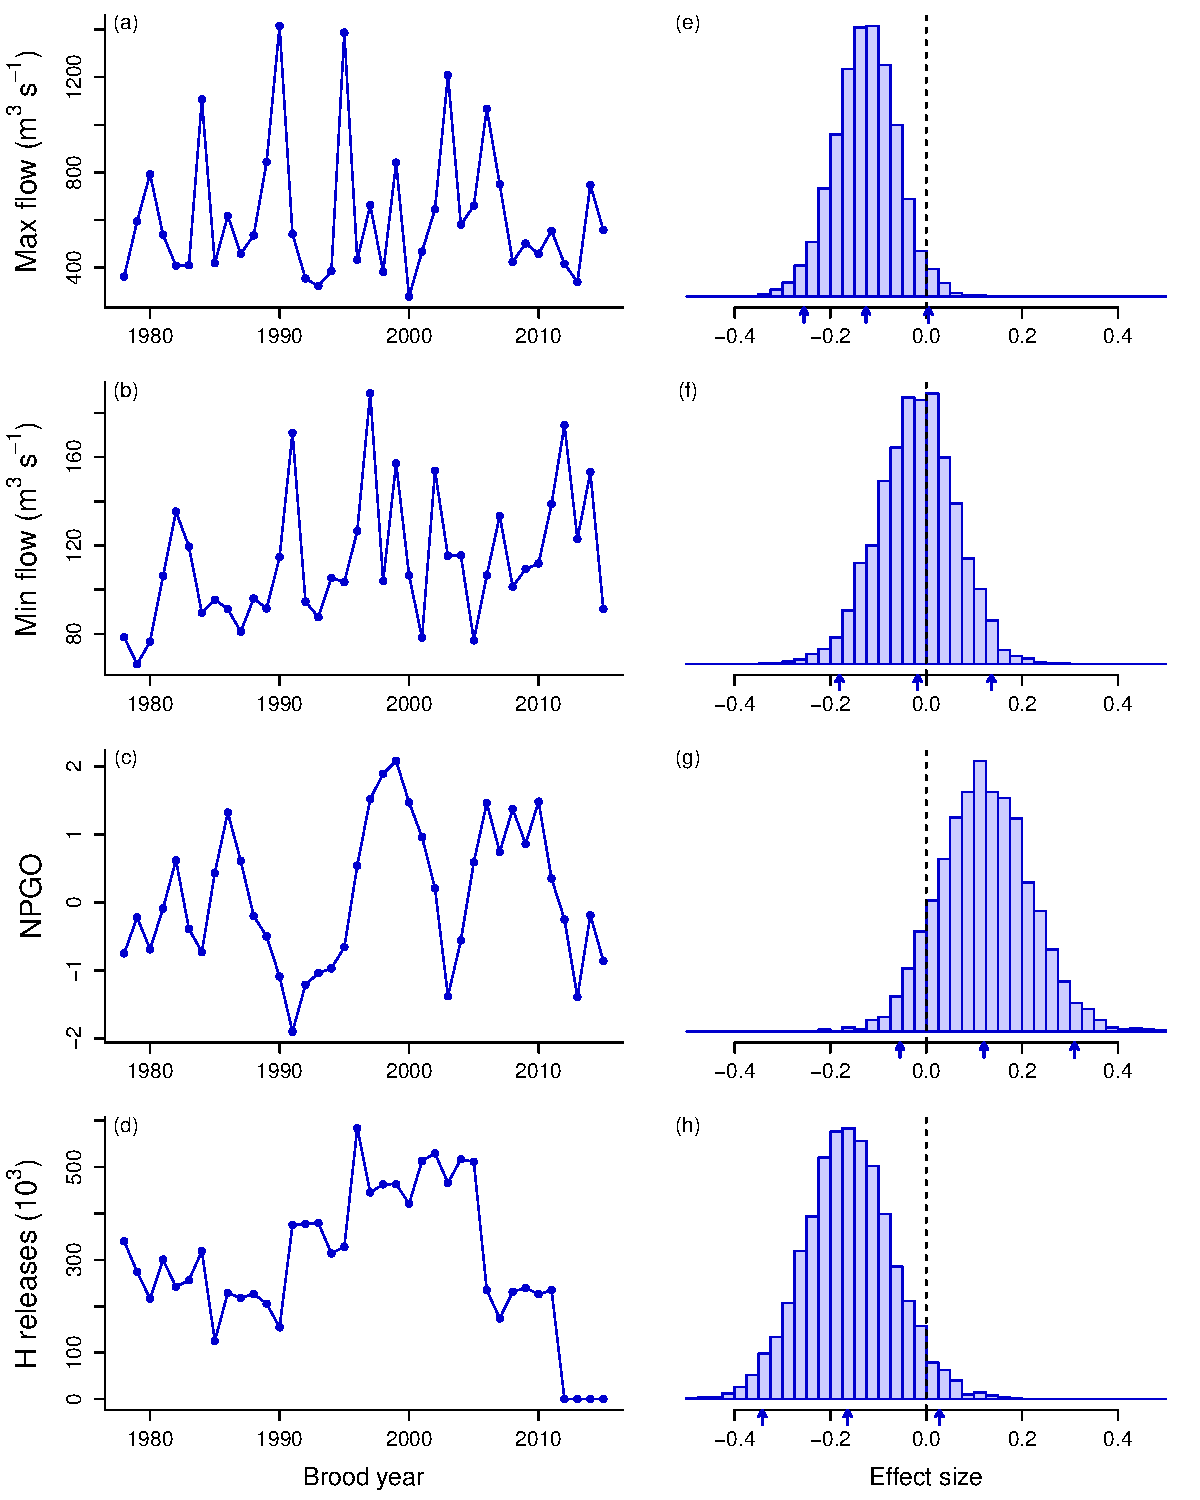
\includegraphics{App_3_Summarize_results_files/figure-latex/fig_4_cov_effects-1} \end{center}

Figure 4: Time series of the environmental covariates used in the model
(a-d), and their estimated effects on population productivity (e-g).
Small arrows under histograms denote 2.5\(^\text{th}\),
50\(^\text{th}\), and 97.5\(^\text{th}\) percentiles of the posterior
distribution.

\hypertarget{fig-5---process-errors}{%
\subsection{Fig 5 - Process errors}\label{fig-5---process-errors}}

Here is the time series of the residuals from the process model. They
represent the population's productivity after accounting for the effects
of density dependence and environmental covariates.

\begin{Shaded}
\begin{Highlighting}[]
\DocumentationTok{\#\# time sequence}
\NormalTok{t\_idx\_a }\OtherTok{\textless{}{-}} \FunctionTok{seq}\NormalTok{(yr\_frst, }\AttributeTok{length.out =}\NormalTok{ n\_yrs}\SpecialCharTok{{-}}\NormalTok{age\_min)}
\DocumentationTok{\#\# plot data}
\NormalTok{p\_dat }\OtherTok{\textless{}{-}}\NormalTok{ mod\_res[, }\FunctionTok{grep}\NormalTok{(}\StringTok{"res\_ln\_Rec"}\NormalTok{, }\FunctionTok{colnames}\NormalTok{(mod\_res))]}
\NormalTok{p\_dat }\OtherTok{\textless{}{-}} \FunctionTok{apply}\NormalTok{(p\_dat, }\DecValTok{2}\NormalTok{, quantile, CI\_vec)}
\NormalTok{yp\_min }\OtherTok{\textless{}{-}} \FunctionTok{min}\NormalTok{(p\_dat)}
\NormalTok{yp\_max }\OtherTok{\textless{}{-}} \FunctionTok{max}\NormalTok{(p\_dat)}
\DocumentationTok{\#\# plot}
\FunctionTok{par}\NormalTok{(}\AttributeTok{mai =} \FunctionTok{c}\NormalTok{(}\FloatTok{0.8}\NormalTok{,}\FloatTok{0.8}\NormalTok{,}\FloatTok{0.1}\NormalTok{,}\FloatTok{0.1}\NormalTok{)) }\CommentTok{\#, omi = c(0,0.2,0.1,0.2))}
\FunctionTok{plot}\NormalTok{(t\_idx\_a, p\_dat[}\DecValTok{3}\NormalTok{,],}
     \AttributeTok{type =} \StringTok{"n"}\NormalTok{,  }\AttributeTok{bty =} \StringTok{"L"}\NormalTok{, }\AttributeTok{xaxt =} \StringTok{"n"}\NormalTok{, }
     \AttributeTok{ylim =} \FunctionTok{c}\NormalTok{(yp\_min,yp\_max),}
     \AttributeTok{xlab =} \StringTok{"Brood year"}\NormalTok{, }\AttributeTok{ylab =} \StringTok{"Process error"}\NormalTok{, }\AttributeTok{main =} \StringTok{""}\NormalTok{,}
     \AttributeTok{cex.lab =} \FloatTok{1.2}\NormalTok{)}
\FunctionTok{abline}\NormalTok{(}\AttributeTok{h =} \DecValTok{0}\NormalTok{, }\AttributeTok{lty =} \StringTok{"dashed"}\NormalTok{)}
\FunctionTok{polygon}\NormalTok{(}\FunctionTok{c}\NormalTok{(t\_idx\_a, }\FunctionTok{rev}\NormalTok{(t\_idx\_a)), }\FunctionTok{c}\NormalTok{(p\_dat[}\DecValTok{3}\NormalTok{,], }\FunctionTok{rev}\NormalTok{(p\_dat[}\DecValTok{1}\NormalTok{,])),}
        \AttributeTok{col =}\NormalTok{ clr, }\AttributeTok{border =} \ConstantTok{NA}\NormalTok{)}
\FunctionTok{lines}\NormalTok{(t\_idx\_a, p\_dat[}\DecValTok{2}\NormalTok{,], }\AttributeTok{col =} \StringTok{"blue3"}\NormalTok{, }\AttributeTok{lwd =} \DecValTok{2}\NormalTok{)}
\FunctionTok{axis}\NormalTok{(}\DecValTok{1}\NormalTok{, }\AttributeTok{at =} \FunctionTok{seq}\NormalTok{(}\DecValTok{1980}\NormalTok{, }\DecValTok{2015}\NormalTok{, }\DecValTok{5}\NormalTok{))}
\end{Highlighting}
\end{Shaded}

\begin{center}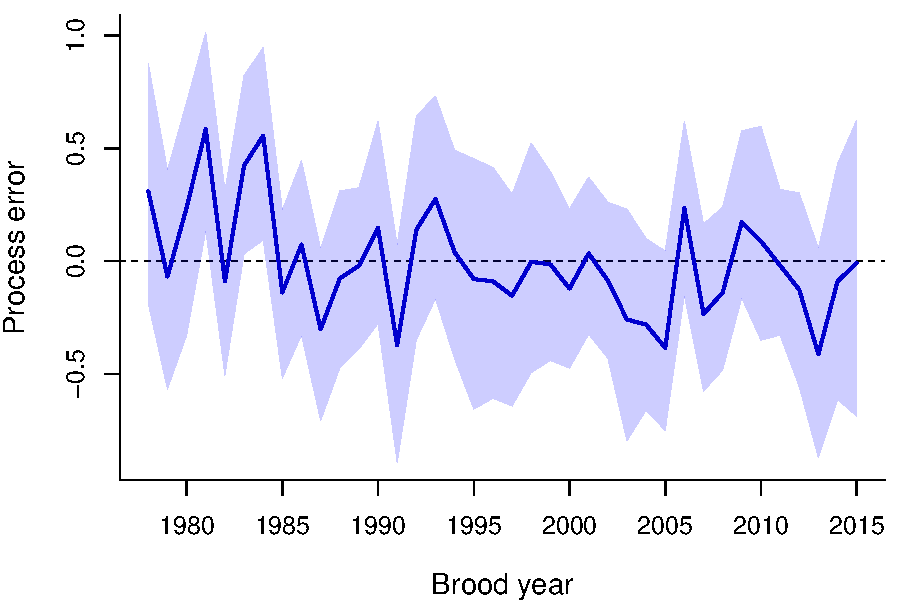
\includegraphics{App_3_Summarize_results_files/figure-latex/fig_5_proc_err-1} \end{center}

Figure 5: Time series of the estimated process errors, which represent
the population's productivity after accounting for the effects of
density dependence and environmental covariates. The solid line is the
median estimate and the shaded region indicates the 95\% credible
interval.

\hypertarget{fig-6---management-reference-points}{%
\subsection{Fig 6 - Management reference
points}\label{fig-6---management-reference-points}}

Here are a number of management reference points.

\begin{Shaded}
\begin{Highlighting}[]
\DocumentationTok{\#\# abbreviations for ref points}
\NormalTok{ref\_names }\OtherTok{\textless{}{-}} \FunctionTok{c}\NormalTok{(}\StringTok{"MSY"}\NormalTok{, }\StringTok{"Smsy"}\NormalTok{, }\StringTok{"Umsy"}\NormalTok{, }\StringTok{"Umax"}\NormalTok{)}
\DocumentationTok{\#\# proportions of MSY to consider}
\NormalTok{yld\_prop }\OtherTok{\textless{}{-}} \FunctionTok{c}\NormalTok{(}\FloatTok{0.75}\NormalTok{, }\FloatTok{0.85}\NormalTok{, }\FloatTok{0.95}\NormalTok{)}
\DocumentationTok{\#\# median values for a \& b}
\NormalTok{aa }\OtherTok{\textless{}{-}}\NormalTok{ mod\_res[, }\FunctionTok{grep}\NormalTok{(}\StringTok{"E\_BH\_a"}\NormalTok{, }\FunctionTok{colnames}\NormalTok{(mod\_res))]}
\NormalTok{alpha }\OtherTok{\textless{}{-}} \FunctionTok{exp}\NormalTok{(aa)}
\NormalTok{mcmc }\OtherTok{\textless{}{-}} \FunctionTok{length}\NormalTok{(aa)}
\NormalTok{beta }\OtherTok{\textless{}{-}}\NormalTok{ mod\_res[, }\FunctionTok{grep}\NormalTok{(}\StringTok{"beta"}\NormalTok{, }\FunctionTok{colnames}\NormalTok{(mod\_res))]}

\DocumentationTok{\#\# empty matrix for ref pts}
\NormalTok{ref\_pts }\OtherTok{\textless{}{-}} \FunctionTok{matrix}\NormalTok{(}\ConstantTok{NA}\NormalTok{, mcmc, }\FunctionTok{length}\NormalTok{(ref\_names))}
\FunctionTok{colnames}\NormalTok{(ref\_pts) }\OtherTok{\textless{}{-}}\NormalTok{ ref\_names}
\DocumentationTok{\#\# spawner series for optimal yield profile}
\NormalTok{SS }\OtherTok{\textless{}{-}} \FunctionTok{seq}\NormalTok{(}\DecValTok{100}\NormalTok{, }\FloatTok{1e4}\NormalTok{, }\DecValTok{100}\NormalTok{)}
\DocumentationTok{\#\# empty matrix for optimal yield profiles}
\NormalTok{OYP }\OtherTok{\textless{}{-}} \FunctionTok{matrix}\NormalTok{(}\DecValTok{0}\NormalTok{, }\FunctionTok{length}\NormalTok{(SS), }\FunctionTok{length}\NormalTok{(yld\_prop))}
\ControlFlowTok{for}\NormalTok{(i }\ControlFlowTok{in} \DecValTok{1}\SpecialCharTok{:}\NormalTok{mcmc) \{}
    \DocumentationTok{\#\# spawners at MSY}
\NormalTok{    ref\_pts[i, }\StringTok{"Smsy"}\NormalTok{] }\OtherTok{\textless{}{-}}\NormalTok{ (alpha[i] }\SpecialCharTok{/}\NormalTok{ beta[i]) }\SpecialCharTok{*} \FunctionTok{sqrt}\NormalTok{(}\DecValTok{1} \SpecialCharTok{/}\NormalTok{ alpha[i]) }\SpecialCharTok{{-}}\NormalTok{ (}\DecValTok{1} \SpecialCharTok{/}\NormalTok{ beta[i])}
    \DocumentationTok{\#\# MSY}
\NormalTok{    ref\_pts[i, }\StringTok{"MSY"}\NormalTok{] }\OtherTok{\textless{}{-}}\NormalTok{ (ref\_pts[i,}\StringTok{"Smsy"}\NormalTok{] }\SpecialCharTok{*}\NormalTok{ alpha[i]) }\SpecialCharTok{/}
\NormalTok{                            (}\DecValTok{1} \SpecialCharTok{+}\NormalTok{ beta[i] }\SpecialCharTok{*}\NormalTok{ ref\_pts[i, }\StringTok{"Smsy"}\NormalTok{]) }\SpecialCharTok{{-}}\NormalTok{ ref\_pts[i, }\StringTok{"Smsy"}\NormalTok{]}
    \DocumentationTok{\#\# harvest rate at MSY}
\NormalTok{    ref\_pts[i, }\StringTok{"Umsy"}\NormalTok{] }\OtherTok{\textless{}{-}} \DecValTok{1} \SpecialCharTok{{-}} \FunctionTok{sqrt}\NormalTok{(}\DecValTok{1} \SpecialCharTok{/}\NormalTok{ alpha[i])}
    \DocumentationTok{\#\# max harvest rate}
\NormalTok{    ref\_pts[i, }\StringTok{"Umax"}\NormalTok{] }\OtherTok{\textless{}{-}} \DecValTok{1} \SpecialCharTok{{-}} \DecValTok{1}\SpecialCharTok{/}\NormalTok{alpha[i]}
    \DocumentationTok{\#\# yield over varying S}
\NormalTok{    yield }\OtherTok{\textless{}{-}}\NormalTok{ ((SS }\SpecialCharTok{*}\NormalTok{ alpha[i]) }\SpecialCharTok{/}\NormalTok{ (}\DecValTok{1} \SpecialCharTok{+}\NormalTok{ beta[i] }\SpecialCharTok{*}\NormalTok{ SS)) }\SpecialCharTok{{-}}\NormalTok{ SS}
    \ControlFlowTok{for}\NormalTok{(j }\ControlFlowTok{in} \DecValTok{1}\SpecialCharTok{:}\FunctionTok{length}\NormalTok{(yld\_prop)) \{}
\NormalTok{        OYP[,j] }\OtherTok{\textless{}{-}}\NormalTok{ OYP[,j] }\SpecialCharTok{+} \DecValTok{1}\SpecialCharTok{*}\NormalTok{(yield }\SpecialCharTok{\textgreater{}}\NormalTok{ yld\_prop[j] }\SpecialCharTok{*}\NormalTok{ ref\_pts[i, }\StringTok{"MSY"}\NormalTok{])}
\NormalTok{    \}}
\NormalTok{\}}
\NormalTok{OYP }\OtherTok{\textless{}{-}}\NormalTok{ OYP}\SpecialCharTok{/}\NormalTok{mcmc}

\DocumentationTok{\#\# Prob of overfishing}
\NormalTok{hh }\OtherTok{\textless{}{-}} \FunctionTok{seq}\NormalTok{(}\DecValTok{100}\NormalTok{)}
\NormalTok{Pr\_over }\OtherTok{\textless{}{-}} \FunctionTok{cbind}\NormalTok{(hh,hh,hh)}
\FunctionTok{colnames}\NormalTok{(Pr\_over) }\OtherTok{\textless{}{-}} \FunctionTok{c}\NormalTok{(}\StringTok{"Umsy75"}\NormalTok{,}\StringTok{"Umsy"}\NormalTok{,}\StringTok{"Umax"}\NormalTok{)}
\ControlFlowTok{for}\NormalTok{(i }\ControlFlowTok{in}\NormalTok{ hh) \{}
\NormalTok{  Pr\_over[i,}\StringTok{"Umsy75"}\NormalTok{] }\OtherTok{\textless{}{-}} \FunctionTok{sum}\NormalTok{(ref\_pts[,}\StringTok{"Umsy"}\NormalTok{] }\SpecialCharTok{*} \FloatTok{0.75} \SpecialCharTok{\textless{}}\NormalTok{ i}\SpecialCharTok{/}\DecValTok{100}\NormalTok{)}\SpecialCharTok{/}\NormalTok{mcmc}
\NormalTok{  Pr\_over[i,}\StringTok{"Umsy"}\NormalTok{] }\OtherTok{\textless{}{-}} \FunctionTok{sum}\NormalTok{(ref\_pts[,}\StringTok{"Umsy"}\NormalTok{] }\SpecialCharTok{\textless{}}\NormalTok{ i}\SpecialCharTok{/}\DecValTok{100}\NormalTok{)}\SpecialCharTok{/}\NormalTok{mcmc}
\NormalTok{  Pr\_over[i,}\StringTok{"Umax"}\NormalTok{] }\OtherTok{\textless{}{-}} \FunctionTok{sum}\NormalTok{(ref\_pts[,}\StringTok{"Umax"}\NormalTok{] }\SpecialCharTok{\textless{}}\NormalTok{ i}\SpecialCharTok{/}\DecValTok{100}\NormalTok{)}\SpecialCharTok{/}\NormalTok{mcmc}
\NormalTok{\}}

\DocumentationTok{\#\# posterior exploitation rate \& spawner abundance}
\NormalTok{aer }\OtherTok{\textless{}{-}}\NormalTok{ Sp\_ts }\OtherTok{\textless{}{-}}\NormalTok{ mod\_res[,}\FunctionTok{grep}\NormalTok{(}\StringTok{"Sp"}\NormalTok{, }\FunctionTok{colnames}\NormalTok{(mod\_res))]}
\ControlFlowTok{for}\NormalTok{(i }\ControlFlowTok{in} \DecValTok{1}\SpecialCharTok{:}\NormalTok{n\_yrs) \{}
\NormalTok{    aer[,i] }\OtherTok{\textless{}{-}}\NormalTok{ dat\_harv[i] }\SpecialCharTok{/}\NormalTok{ (dat\_harv[i] }\SpecialCharTok{+}\NormalTok{ Sp\_ts[,i]) }
\NormalTok{\}}
\end{Highlighting}
\end{Shaded}

\begin{Shaded}
\begin{Highlighting}[]
\FunctionTok{layout}\NormalTok{(}\FunctionTok{matrix}\NormalTok{(}\FunctionTok{c}\NormalTok{(}\DecValTok{2}\NormalTok{, }\DecValTok{1}\NormalTok{, }\DecValTok{4}\NormalTok{, }\DecValTok{3}\NormalTok{), }\DecValTok{2}\NormalTok{, }\DecValTok{2}\NormalTok{), }\AttributeTok{heights =} \FunctionTok{c}\NormalTok{(}\DecValTok{1}\NormalTok{, }\DecValTok{5}\NormalTok{))}
\NormalTok{yoffSet }\OtherTok{\textless{}{-}} \FloatTok{0.10}
\NormalTok{yoffSet }\OtherTok{\textless{}{-}} \FloatTok{0.05}

\NormalTok{clr\_f6 }\OtherTok{\textless{}{-}} \FunctionTok{c}\NormalTok{(}\StringTok{"slateblue"}\NormalTok{,}\StringTok{"blue"}\NormalTok{,}\StringTok{"darkblue"}\NormalTok{)}

\FunctionTok{par}\NormalTok{(}\AttributeTok{mai=}\FunctionTok{c}\NormalTok{(}\FloatTok{0.9}\NormalTok{, }\FloatTok{0.9}\NormalTok{, }\DecValTok{0}\NormalTok{, }\DecValTok{0}\NormalTok{), }\AttributeTok{omi=}\FunctionTok{c}\NormalTok{(}\DecValTok{0}\NormalTok{, }\DecValTok{0}\NormalTok{, }\FloatTok{0.1}\NormalTok{, }\FloatTok{0.1}\NormalTok{))}

\DocumentationTok{\#\# (a) Optimal yield profile}
\FunctionTok{matplot}\NormalTok{(SS, OYP, }\AttributeTok{type=}\StringTok{"l"}\NormalTok{, }\AttributeTok{lty=}\StringTok{"solid"}\NormalTok{,  }\AttributeTok{ylim=}\FunctionTok{c}\NormalTok{(}\DecValTok{0}\NormalTok{,}\DecValTok{1}\NormalTok{),}
        \AttributeTok{col=}\NormalTok{clr\_f6, }\AttributeTok{lwd=}\DecValTok{2}\NormalTok{,}
        \AttributeTok{xlab =} \StringTok{"Spawners"}\NormalTok{, }\AttributeTok{ylab =} \StringTok{"Probability of X\% of MSY"}\NormalTok{, }\AttributeTok{main =} \StringTok{""}\NormalTok{,}
        \AttributeTok{las=}\DecValTok{1}\NormalTok{, }\AttributeTok{cex.lab=}\FloatTok{1.2}\NormalTok{)}
\FunctionTok{points}\NormalTok{(}\AttributeTok{x =} \FunctionTok{c}\NormalTok{(}\DecValTok{5500}\NormalTok{, }\DecValTok{4300}\NormalTok{, }\DecValTok{2500}\NormalTok{), }\AttributeTok{y =} \FunctionTok{c}\NormalTok{(}\FloatTok{0.4}\NormalTok{, }\FloatTok{0.5}\NormalTok{, }\FloatTok{0.55}\NormalTok{),}
       \AttributeTok{pch =} \DecValTok{21}\NormalTok{, }\AttributeTok{cex =} \FloatTok{3.5}\NormalTok{,}
       \AttributeTok{col =} \StringTok{"white"}\NormalTok{, }\AttributeTok{bg =} \StringTok{"white"}\NormalTok{)}
\FunctionTok{text}\NormalTok{(}\AttributeTok{x =} \FunctionTok{c}\NormalTok{(}\DecValTok{5500}\NormalTok{, }\DecValTok{4300}\NormalTok{, }\DecValTok{2500}\NormalTok{), }\AttributeTok{y =} \FunctionTok{c}\NormalTok{(}\FloatTok{0.4}\NormalTok{, }\FloatTok{0.5}\NormalTok{, }\FloatTok{0.55}\NormalTok{), }\FunctionTok{paste0}\NormalTok{(yld\_prop}\SpecialCharTok{*}\DecValTok{100}\NormalTok{, }\StringTok{"\%"}\NormalTok{),}
     \AttributeTok{col=}\FunctionTok{c}\NormalTok{(}\StringTok{"slateblue"}\NormalTok{,}\StringTok{"blue"}\NormalTok{,}\StringTok{"darkblue"}\NormalTok{), }\AttributeTok{cex=}\FloatTok{0.7}\NormalTok{)}
\FunctionTok{text}\NormalTok{(}\AttributeTok{x =} \FunctionTok{par}\NormalTok{()}\SpecialCharTok{$}\NormalTok{usr[}\DecValTok{1}\NormalTok{] }\SpecialCharTok{+}\NormalTok{ xoffSet }\SpecialCharTok{*} \FunctionTok{diff}\NormalTok{(}\FunctionTok{par}\NormalTok{()}\SpecialCharTok{$}\NormalTok{usr[}\DecValTok{1}\SpecialCharTok{:}\DecValTok{2}\NormalTok{]),}
     \AttributeTok{y =} \FunctionTok{par}\NormalTok{()}\SpecialCharTok{$}\NormalTok{usr[}\DecValTok{4}\NormalTok{] }\SpecialCharTok{{-}}\NormalTok{ yoffSet }\SpecialCharTok{*} \FunctionTok{diff}\NormalTok{(}\FunctionTok{par}\NormalTok{()}\SpecialCharTok{$}\NormalTok{usr[}\DecValTok{3}\SpecialCharTok{:}\DecValTok{4}\NormalTok{]),}
     \StringTok{"(a)"}\NormalTok{)}
\DocumentationTok{\#\# marginal histogram of posterior spawner abundances}
\FunctionTok{par}\NormalTok{(}\AttributeTok{mai=}\FunctionTok{c}\NormalTok{(}\DecValTok{0}\NormalTok{, }\FloatTok{0.9}\NormalTok{, }\FloatTok{0.05}\NormalTok{, }\DecValTok{0}\NormalTok{))}
\FunctionTok{hist}\NormalTok{(Sp\_ts[Sp\_ts}\SpecialCharTok{\textless{}}\FloatTok{1e4}\NormalTok{], }\AttributeTok{breaks =} \DecValTok{40}\NormalTok{,}
     \AttributeTok{col =}\NormalTok{ clr, }\AttributeTok{border =} \StringTok{"blue3"}\NormalTok{, }
     \AttributeTok{yaxs =} \StringTok{"i"}\NormalTok{, }\AttributeTok{xaxt =} \StringTok{"n"}\NormalTok{, }\AttributeTok{yaxt =} \StringTok{"n"}\NormalTok{,}
     \AttributeTok{main =} \StringTok{""}\NormalTok{, }\AttributeTok{ylab =} \StringTok{""}\NormalTok{)}

\DocumentationTok{\#\# (b) Probability of overfishing}
\FunctionTok{par}\NormalTok{(}\AttributeTok{mai=}\FunctionTok{c}\NormalTok{(}\FloatTok{0.9}\NormalTok{, }\FloatTok{0.9}\NormalTok{, }\DecValTok{0}\NormalTok{, }\DecValTok{0}\NormalTok{))}
\FunctionTok{matplot}\NormalTok{(Pr\_over, }\AttributeTok{type =} \StringTok{"l"}\NormalTok{, }\AttributeTok{lwd =} \DecValTok{2}\NormalTok{, }\AttributeTok{lty =} \StringTok{"solid"}\NormalTok{,}
        \AttributeTok{col =}\NormalTok{ clr\_f6, }
        \AttributeTok{ylab=}\StringTok{"Probability of overfishing"}\NormalTok{, }
        \AttributeTok{xlab=}\StringTok{"Harvest rate"}\NormalTok{, }\AttributeTok{xaxt=}\StringTok{"n"}\NormalTok{,}
        \AttributeTok{las =} \DecValTok{1}\NormalTok{, }\AttributeTok{cex.lab =} \FloatTok{1.2}\NormalTok{)}
\FunctionTok{axis}\NormalTok{(}\DecValTok{1}\NormalTok{, }\FunctionTok{seq}\NormalTok{(}\DecValTok{0}\NormalTok{,}\DecValTok{100}\NormalTok{,}\DecValTok{20}\NormalTok{), }\FunctionTok{seq}\NormalTok{(}\DecValTok{0}\NormalTok{,}\DecValTok{100}\NormalTok{,}\DecValTok{20}\NormalTok{)}\SpecialCharTok{/}\DecValTok{100}\NormalTok{)}
\NormalTok{x\_lp }\OtherTok{\textless{}{-}} \FunctionTok{c}\NormalTok{(}\DecValTok{0}\NormalTok{, }\DecValTok{0}\NormalTok{, }\DecValTok{0}\NormalTok{)}
\ControlFlowTok{for}\NormalTok{(i }\ControlFlowTok{in} \DecValTok{1}\SpecialCharTok{:}\FunctionTok{length}\NormalTok{(x\_lp)) \{}
\NormalTok{  x\_lp[i] }\OtherTok{\textless{}{-}} \FunctionTok{max}\NormalTok{(}\FunctionTok{which}\NormalTok{(}\FunctionTok{abs}\NormalTok{(Pr\_over[,i] }\SpecialCharTok{{-}} \FloatTok{0.5}\NormalTok{) }\SpecialCharTok{\textless{}=} \FloatTok{0.05}\NormalTok{))}
\NormalTok{\}}
\FunctionTok{points}\NormalTok{(}\AttributeTok{x =}\NormalTok{ x\_lp, }\AttributeTok{y =} \FunctionTok{rep}\NormalTok{(}\FloatTok{0.5}\NormalTok{, }\DecValTok{3}\NormalTok{), }\AttributeTok{pch =} \DecValTok{21}\NormalTok{, }\AttributeTok{cex =} \DecValTok{4}\NormalTok{,}
       \AttributeTok{col =} \StringTok{"white"}\NormalTok{, }\AttributeTok{bg =} \StringTok{"white"}\NormalTok{)}
\FunctionTok{text}\NormalTok{(}\AttributeTok{x =}\NormalTok{ x\_lp, }\AttributeTok{y =} \FloatTok{0.5}\NormalTok{, }\FunctionTok{expression}\NormalTok{(U[M75], U[MSY], U[Max]),}
     \AttributeTok{col =} \FunctionTok{c}\NormalTok{(}\StringTok{"slateblue"}\NormalTok{, }\StringTok{"blue"}\NormalTok{, }\StringTok{"darkblue"}\NormalTok{), }\AttributeTok{cex =} \FloatTok{0.8}\NormalTok{)}
\FunctionTok{text}\NormalTok{(}\AttributeTok{x =} \FunctionTok{par}\NormalTok{()}\SpecialCharTok{$}\NormalTok{usr[}\DecValTok{1}\NormalTok{] }\SpecialCharTok{+}\NormalTok{ xoffSet }\SpecialCharTok{*} \FunctionTok{diff}\NormalTok{(}\FunctionTok{par}\NormalTok{()}\SpecialCharTok{$}\NormalTok{usr[}\DecValTok{1}\SpecialCharTok{:}\DecValTok{2}\NormalTok{]),}
     \AttributeTok{y =} \FunctionTok{par}\NormalTok{()}\SpecialCharTok{$}\NormalTok{usr[}\DecValTok{4}\NormalTok{] }\SpecialCharTok{{-}}\NormalTok{ yoffSet }\SpecialCharTok{*} \FunctionTok{diff}\NormalTok{(}\FunctionTok{par}\NormalTok{()}\SpecialCharTok{$}\NormalTok{usr[}\DecValTok{3}\SpecialCharTok{:}\DecValTok{4}\NormalTok{]),}
     \StringTok{"(b)"}\NormalTok{)}
\DocumentationTok{\#\# marginal histogram of posterior harvest rates}
\FunctionTok{par}\NormalTok{(}\AttributeTok{mai =} \FunctionTok{c}\NormalTok{(}\DecValTok{0}\NormalTok{ ,}\FloatTok{0.9}\NormalTok{, }\FloatTok{0.05}\NormalTok{, }\DecValTok{0}\NormalTok{))}
\FunctionTok{hist}\NormalTok{(aer, }\AttributeTok{breaks =} \FunctionTok{seq}\NormalTok{(}\DecValTok{0}\NormalTok{, }\DecValTok{40}\NormalTok{)}\SpecialCharTok{/}\DecValTok{40}\NormalTok{,}
     \AttributeTok{col =}\NormalTok{ clr, }\AttributeTok{border =} \StringTok{"blue3"}\NormalTok{,}
     \AttributeTok{yaxs =} \StringTok{"i"}\NormalTok{, }\AttributeTok{xaxt =} \StringTok{"n"}\NormalTok{, }\AttributeTok{yaxt =} \StringTok{"n"}\NormalTok{,}
     \AttributeTok{main =} \StringTok{""}\NormalTok{, }\AttributeTok{ylab =} \StringTok{""}\NormalTok{)}
\end{Highlighting}
\end{Shaded}

\begin{center}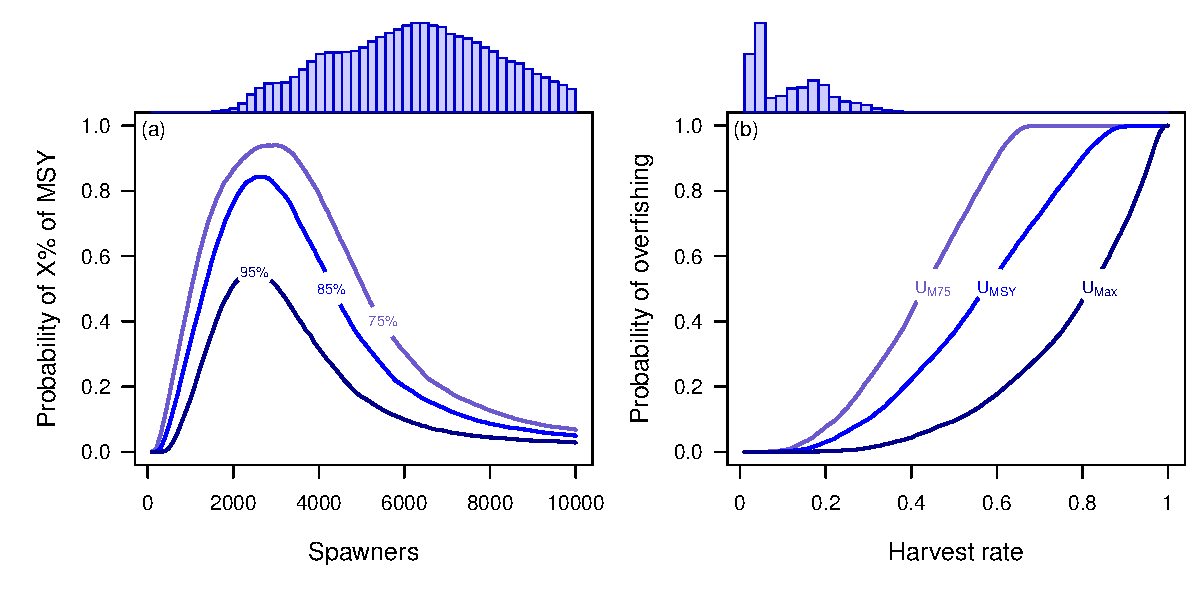
\includegraphics{App_3_Summarize_results_files/figure-latex/fig_6_ref_pts-1} \end{center}

Figure 6: Plots of (a) the probability that a given number of spawners
produces average yields achieving 95\%, 85\%, or 75\% of the estimated
maximum sustainable yield (MSY); and (b) the cumulative probability of
overfishing the population, based on harvest rates equal to those at
75\% of MSY, at MSY, and at the maximum per recruit. The histograms
above (a) and (b) are distributions of the posterior estimates for the
number of spawners and harvest rates, respectively; the histogram in (a)
has been truncated at \(10^4\).

\newpage

\hypertarget{miscellaneous-results}{%
\section{Miscellaneous results}\label{miscellaneous-results}}

Here are summaries of the posterior distributions for \(\alpha\) and
\(K\).

\begin{Shaded}
\begin{Highlighting}[]
\DocumentationTok{\#\# intrinsic productivity}
\FunctionTok{round}\NormalTok{(alphaCI, }\DecValTok{2}\NormalTok{)}
\end{Highlighting}
\end{Shaded}

\begin{verbatim}
##  2.5%   50% 97.5% 
##  1.37  4.80 41.39
\end{verbatim}

\begin{Shaded}
\begin{Highlighting}[]
\DocumentationTok{\#\# carrying capacity}
\FunctionTok{round}\NormalTok{(R\_b\_CI, }\DecValTok{2}\NormalTok{)}
\end{Highlighting}
\end{Shaded}

\begin{verbatim}
##  2.5%   50% 97.5% 
##  5.91  7.70 12.79
\end{verbatim}

Here is a summary of the covariate effect sizes.

\begin{Shaded}
\begin{Highlighting}[]
\NormalTok{gamma\_CI }\OtherTok{\textless{}{-}} \FunctionTok{apply}\NormalTok{(c\_est, }\DecValTok{2}\NormalTok{, quantile, }\FunctionTok{c}\NormalTok{(}\FloatTok{2.5}\NormalTok{, }\DecValTok{5}\NormalTok{, }\DecValTok{50}\NormalTok{, }\DecValTok{95}\NormalTok{, }\FloatTok{97.5}\NormalTok{)}\SpecialCharTok{/}\DecValTok{100}\NormalTok{)}
\FunctionTok{t}\NormalTok{(}\FunctionTok{round}\NormalTok{(gamma\_CI, }\DecValTok{2}\NormalTok{))}
\end{Highlighting}
\end{Shaded}

\begin{verbatim}
##           2.5%    5%   50%   95% 97.5%
## gamma[1] -0.26 -0.23 -0.13 -0.02  0.00
## gamma[2] -0.18 -0.15 -0.02  0.11  0.14
## gamma[3] -0.05 -0.03  0.12  0.28  0.31
## gamma[4] -0.34 -0.31 -0.16 -0.01  0.03
\end{verbatim}

\end{document}
